\chapter{系统构建与技术实现}
\section{页面设计总览}
本章阐述系统的具体构建过程。参考同类毕业论文先页面、再日志、再存储的组织顺序，本章首先介绍四个核心页面：系统首页、模型配置、能源分析与决策轨迹。页面统一采用Vue与Element UI实现\cite{vue2024,elementui2024}，图表采用ECharts绘制\cite{echarts2024}。后文4.5节单列前端系统功能介绍并预留截图位置，5.1节将介绍Postman如何保障接口契约\cite{postman2024}。

\subsection{系统首页设计}
用户登录后首先进入系统首页。顶部导航分为系统首页、模型配置、能源分析与决策轨迹四个板块，右上角为用户菜单。页面中部大标题点明建筑群节能控制主题，旁设新建仿真任务快捷按钮，便于新用户快速定位功能入口。首页同时聚合社区KPI卡片，默认加载最近一次完成任务的成本、碳排放与峰值指标，无需跳转页面即可获得整体概览。

\begin{figure}[htb]
    \centering
    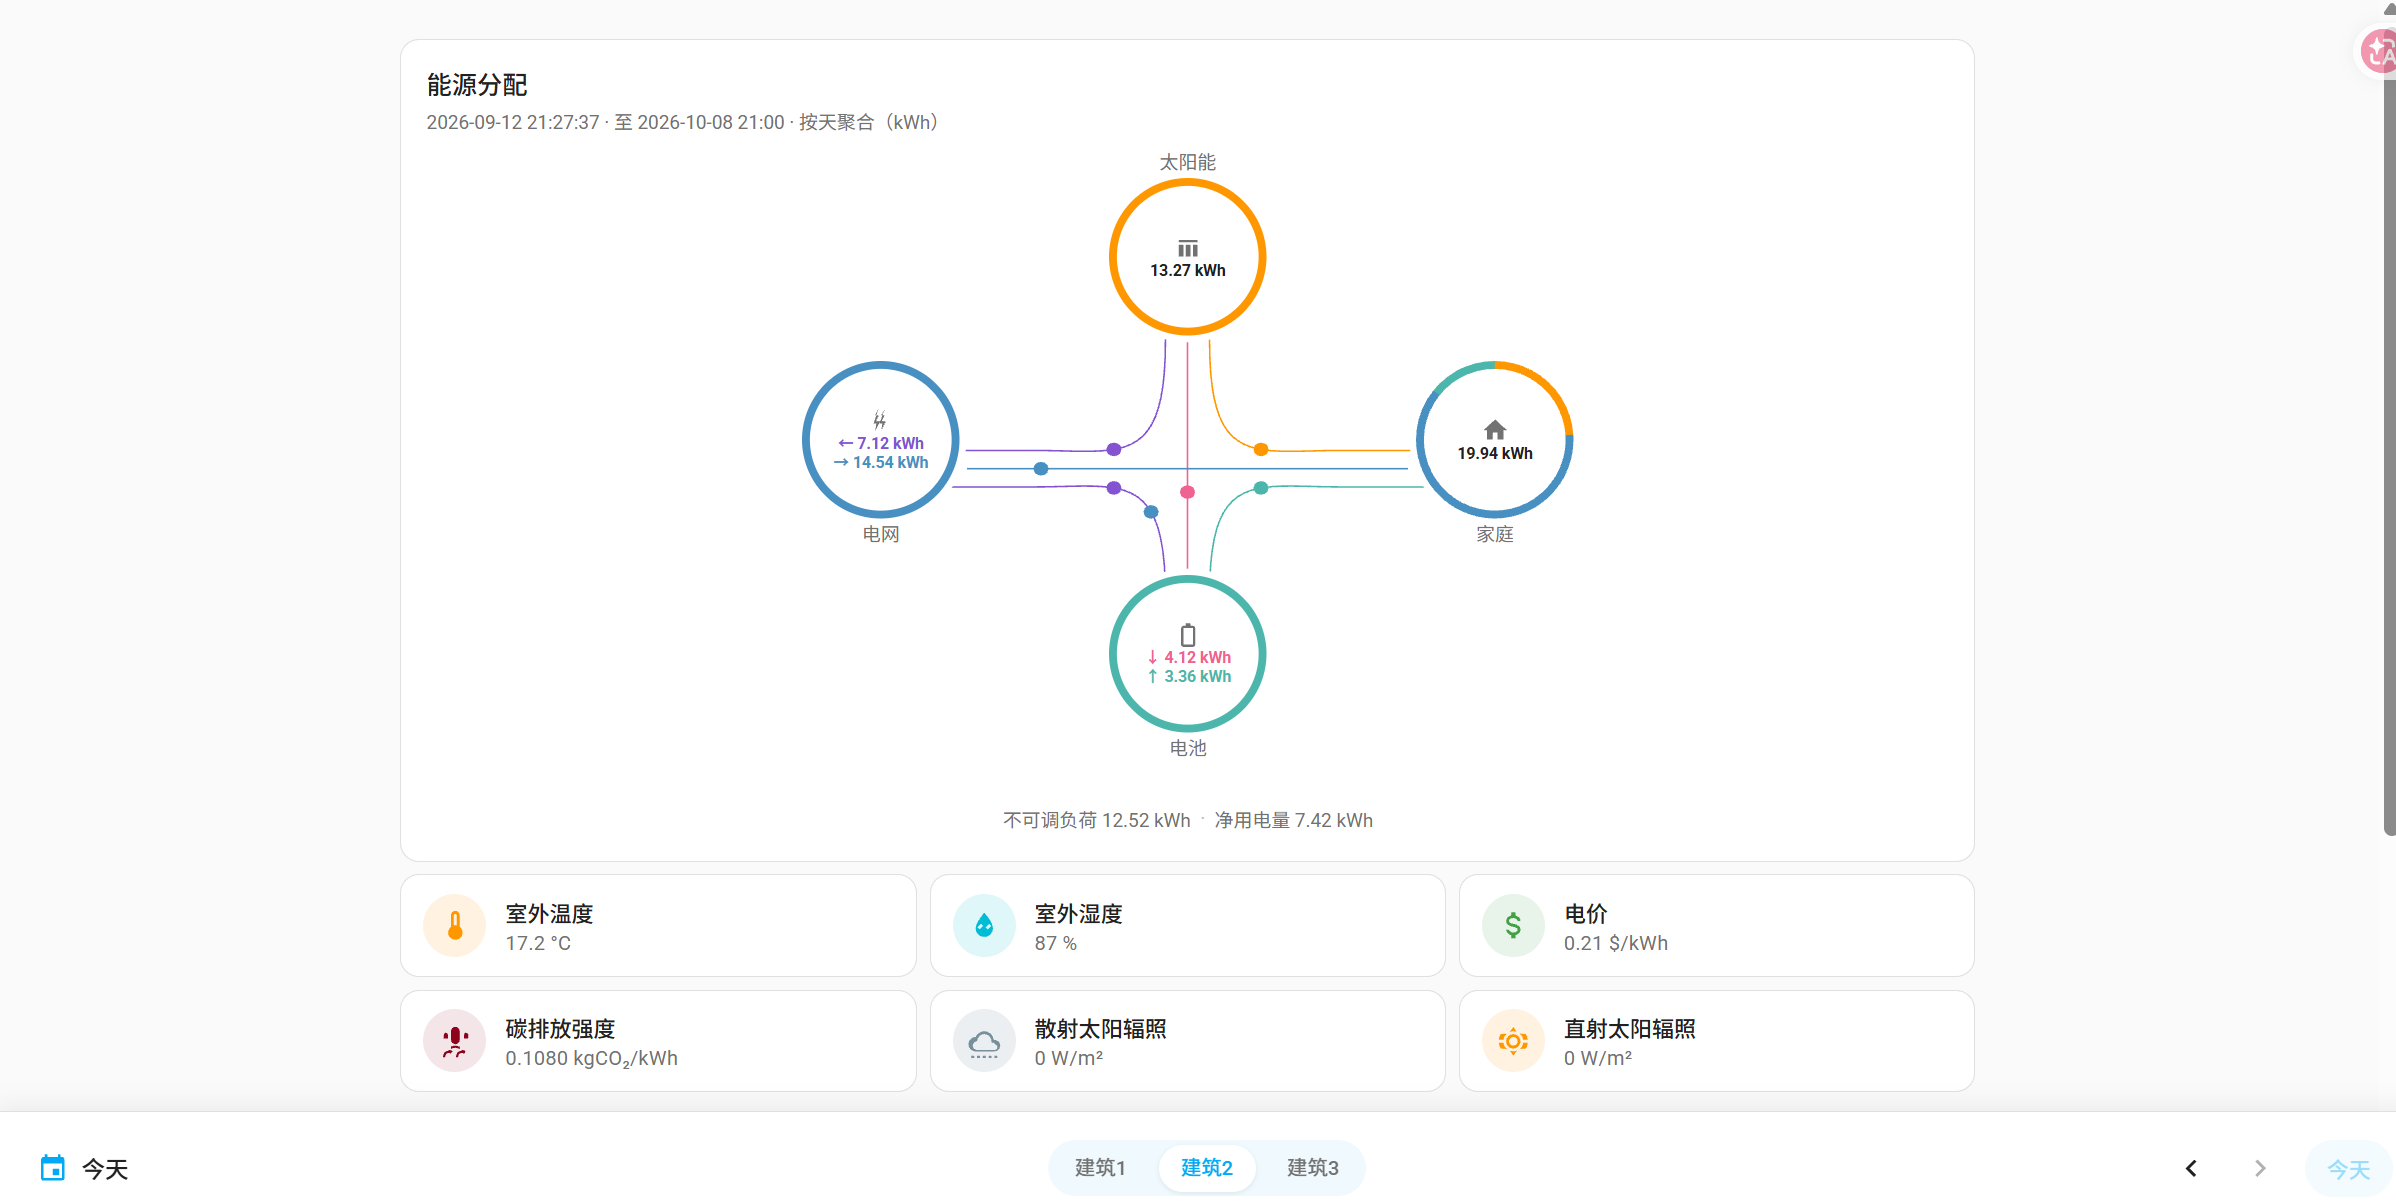
\includegraphics[width=0.85\textwidth]{./images/image/首页.jpg}
    \centering\bicaption{系统首页}{Home page}
    \label{系统首页界面}
\end{figure}

\subsection{算法与数据集配置页面设计}
配置页面的核心是一张带校验规则的表单。字段包括控制器类型、数据集、仿真步数、残差系数、动作掩码、安全投影开关与多智能体模型文件路径。选择纯基线控制时残差相关项自动隐藏；选择残差强化学习模式时模型文件为必填项且需校验数据集兼容性。校验基于表单规则实现\cite{elementui2024}，填写错误时前端直接拦截、不发送请求。提交成功后任务进入列表并实时可见。
\begin{figure}[htb]
    \centering
    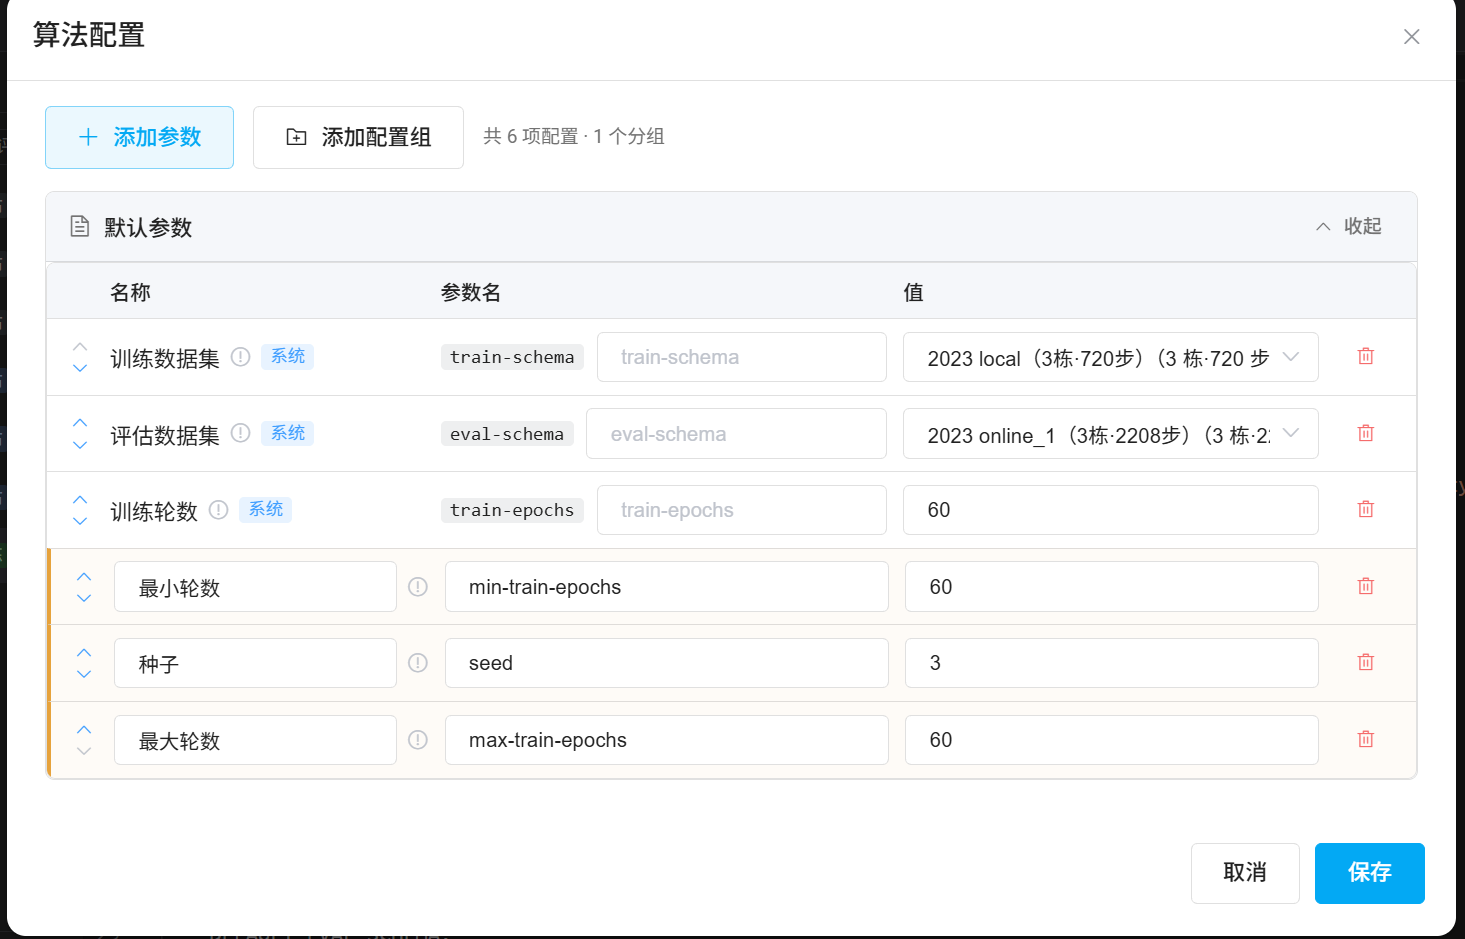
\includegraphics[width=0.85\textwidth]{./images/image/算法配置页.jpg}
    \centering\bicaption{模型配置页}{Model config page}
    \label{模型配置页面}
\end{figure}

\subsection{能源与KPI分析页面设计}
分析页面采用分块多图布局。折线图展示负荷与电价随时间步的变化，柱状图比较不同算法的KPI，雷达图呈现五维指标权衡。首次进入页面自动加载默认任务，检索框支持按任务标识回溯历史任务。全平台配色统一：电网蓝、光伏橙、电池青绿，多任务对比时不会发生混淆。
\begin{figure}[htb]
    \centering
    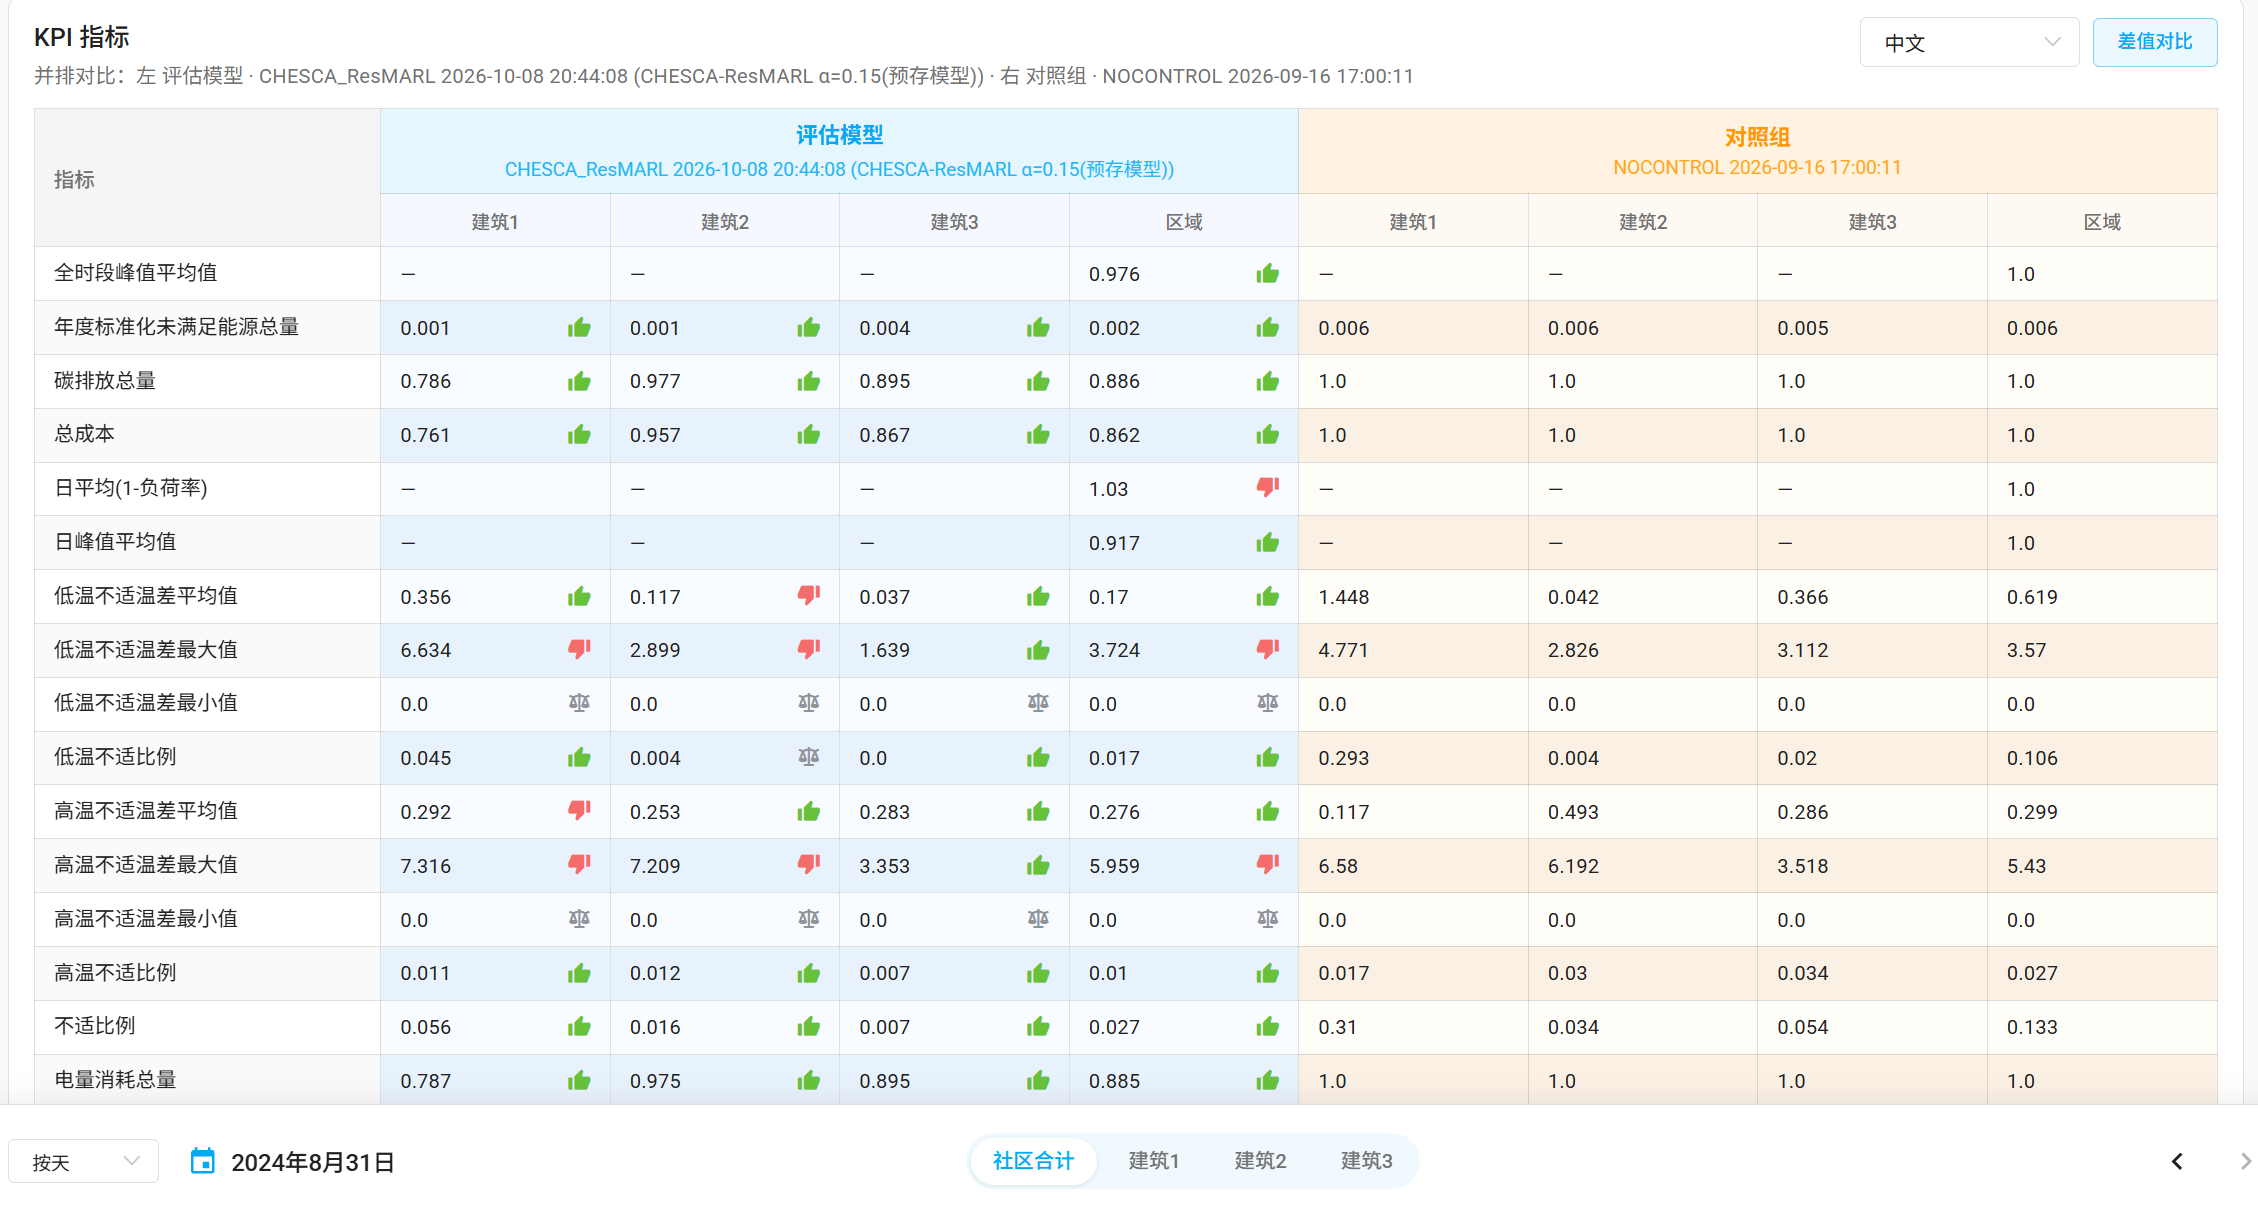
\includegraphics[width=0.85\textwidth]{./images/image/指标对比.jpg}
    \centering\bicaption{能源KPI分析页}{KPI analysis page}
    \label{能源KPI分析页面}
\end{figure}

\subsection{决策轨迹页面设计}
轨迹页面按时间步读取决策推演日志与决策记录，将基线动作、原始残差、掩码、投影后动作、SOC与舒适度状态绘制于同一时间轴。定位至峰值时段后，可直接观察残差是否被安全层约束，较仅查看最终指标更具诊断价值。该页面由轨迹面板、决策记录日志与残差增量展示等一组组件协作实现，分别负责轨迹主视图渲染、逐步决策记录回放与各通道残差增量的可视化。
\begin{figure}[htb]
    \centering
    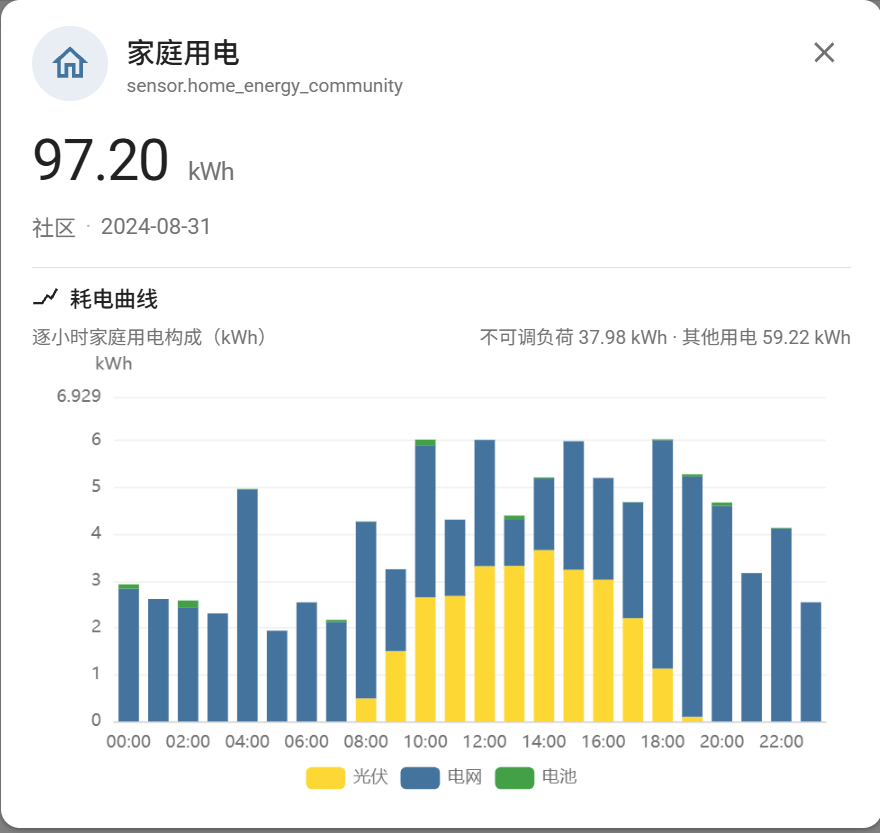
\includegraphics[width=0.85\textwidth]{./images/image/环境状态1.jpg}
    \centering\bicaption{决策轨迹页}{Decision trace page}
    \label{决策轨迹页面}
\end{figure}

\section{日志的自动化与规范化管理}
日志部分需首先交代现状：项目目前尚未部署独立日志平台，采用文件日志、任务目录归档与数据库状态字段相结合的组合方案。Python标准输出重定向至任务目录，配置、指标与轨迹文件按任务标识隔离；Java端读取退出码更新任务状态，解析失败时保留原始行并标注原因。问题排查主要检查三个文件：运行日志、算法指标与决策推演日志。

日志规范分为三个环节。第一，自动化解析：日志中混合配置、奖励与指标等信息，采用正则表达式提取字段，提取失败时记录原始行与原因，不做静默丢弃。第二，规范导出：解析结果按结构化文件格式落盘，字段名与数据库保持一致，时间步从0开始连续编号，缺失步需显式标注。第三，持久化：明细数据经事务写入数据库，指标聚合结果写入指标汇总数据，明细数据保留在文件中，数据库仅保存索引。并发任务采用多线程或异步写入，互不阻塞。

集中式日志方案作为备选，当前阶段不强制部署。待日志规模增长后接入ELK或Loki\cite{elk2024}：采集组件采集各节点日志，按任务标识、控制器类型与数据集类型打标签，Kibana按任务查询全链路日志。字段规范在本节固化，后续仅需增加采集组件，无需返工。日志流水线如图\figref{日志流水线图}所示。
\begin{figure}[htb]
    \centering
    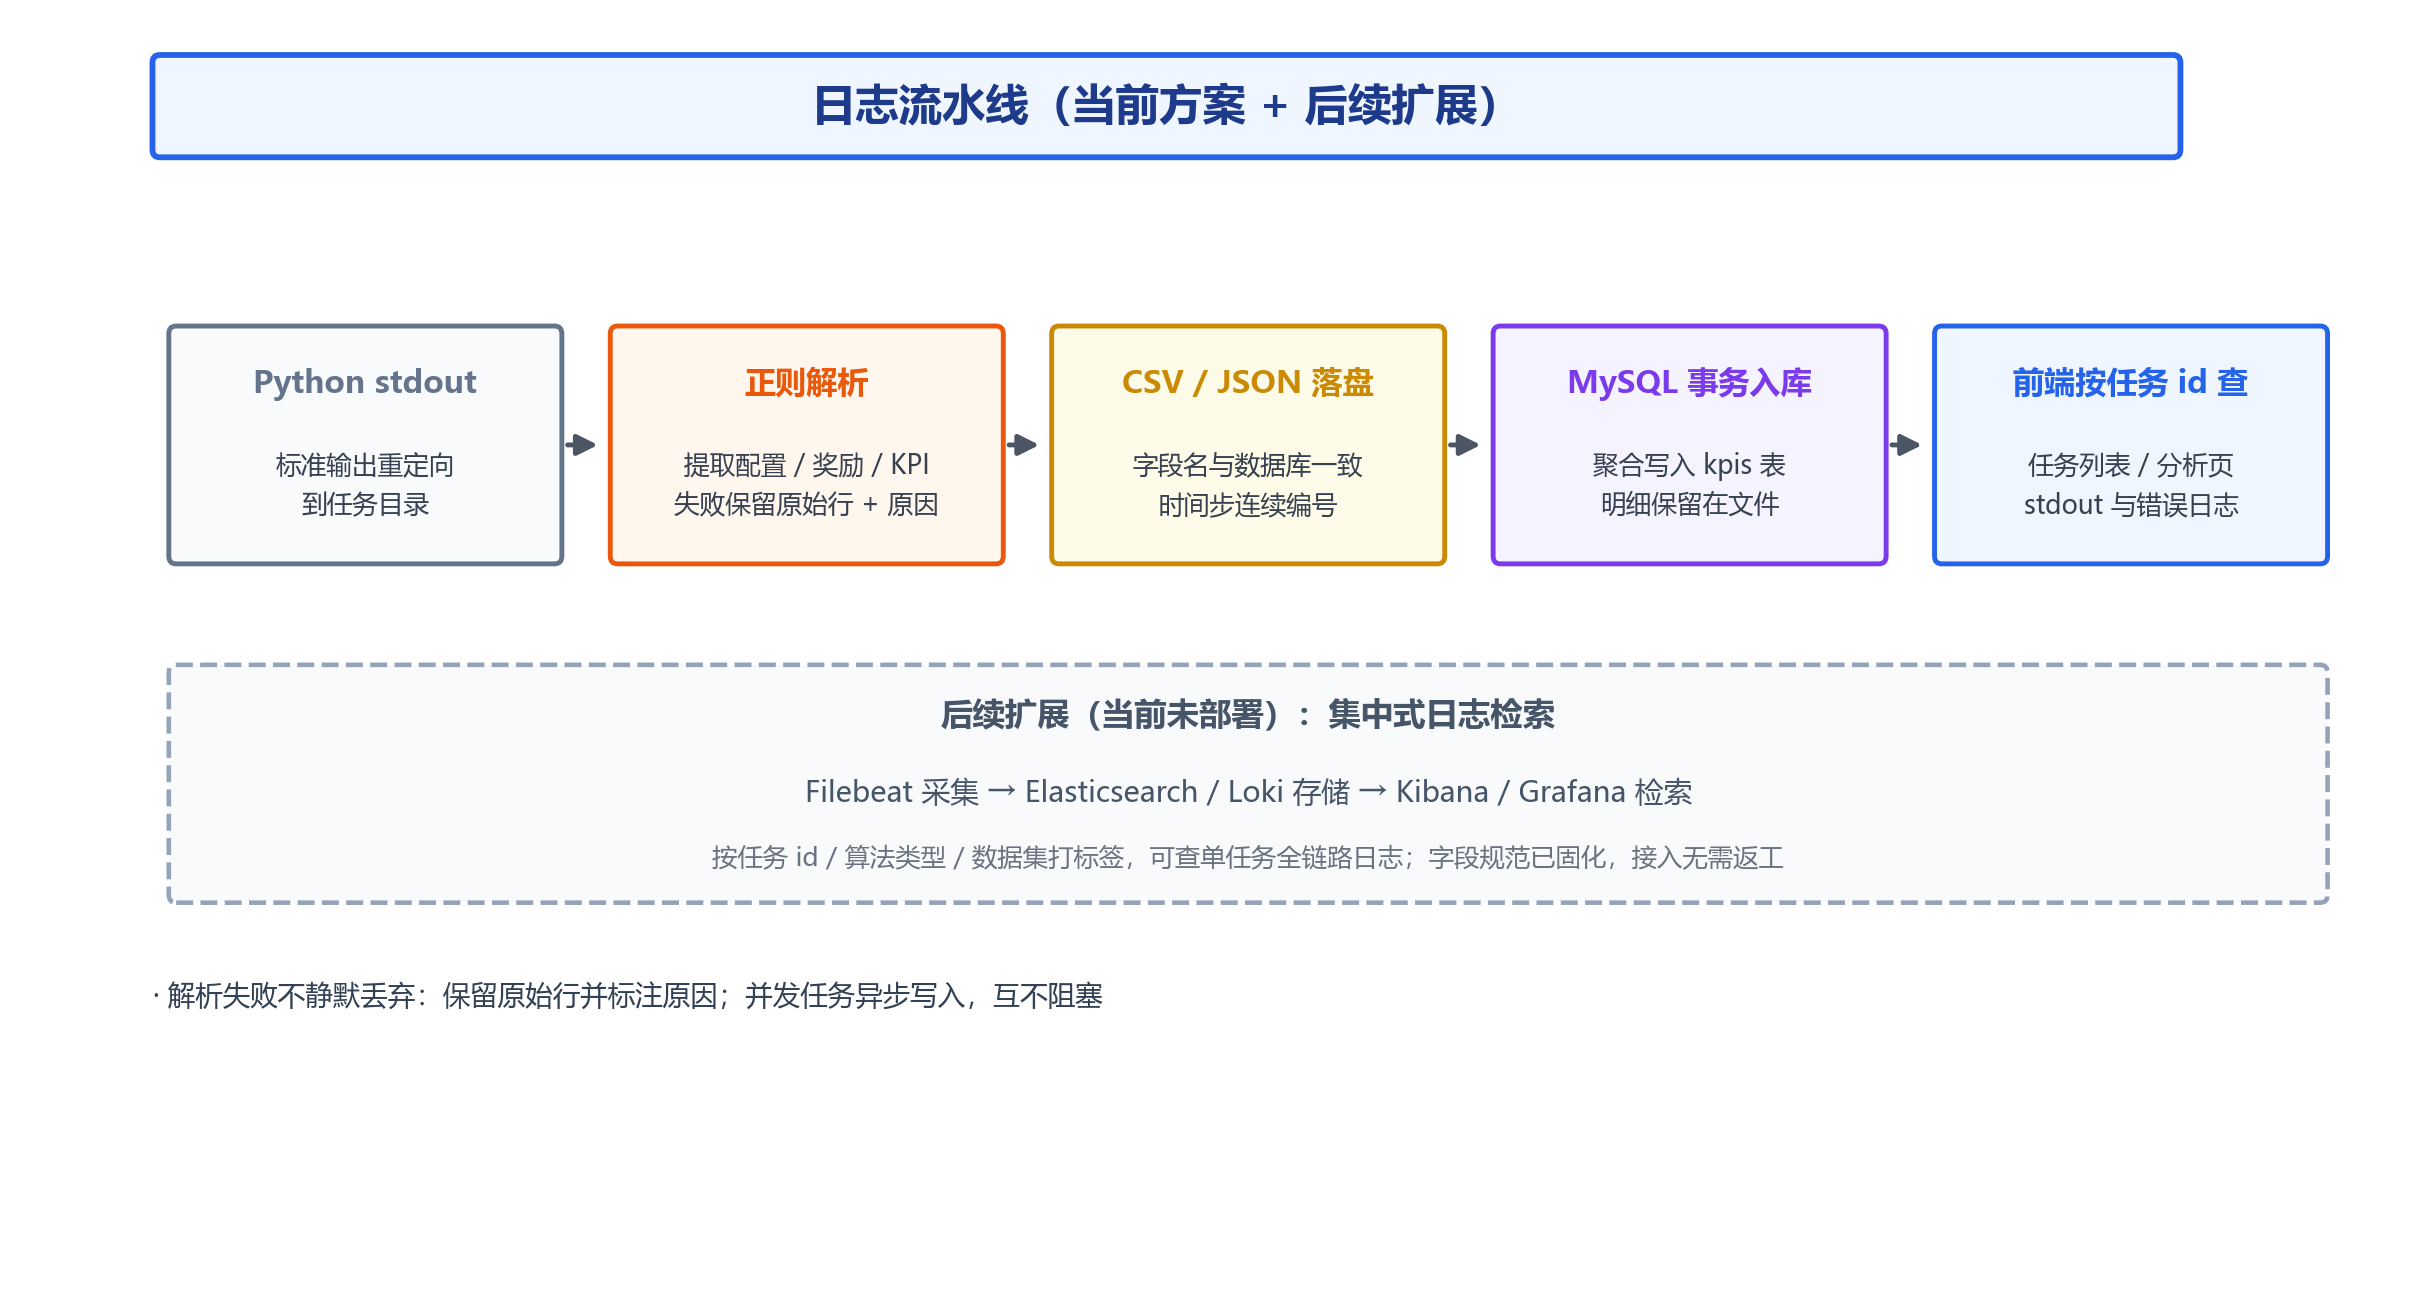
\includegraphics[width=0.92\textwidth]{./images/pictures/日志流水线图.png}
    \centering\bicaption{日志流水线图}{Log pipeline}
    \label{日志流水线图}
\end{figure}

\section{数据库设计与实现}
数据库采用MySQL 8.0 InnoDB引擎，字符集\texttt{utf8mb4}。数据表按业务功能分为五组：建筑时序、环境时序、算法脚本与任务、评价指标、配置与目录。

（1）建筑时序表，如表\ref{tab:building-table}所示。各建筑对应的表结构相同，按建筑区分存储，存储月份、小时、日类型、夏令时、室内温湿度、未满足冷设定点差、不可转移负荷、热水/冷热需求、光伏发电、占用人数、设定点与HVAC模式。主键按时间步连续编号，与CityLearn观测一一对应，前端曲线直接读取。
\begin{table}[h!]
    \centering\bicaption{建筑时序表设计}{Design of building time-series table}
    \label{tab:building-table}
    \begin{tabular}{P{14em}P{6em}P{4em}P{8em}}
        \toprule
        字段名 & 数据类型 & 非空 & 注释 \\\midrule
        id & bigint & 是 & 时间步主键 \\
        month & int & 否 & 月份 \\
        hour & int & 否 & 小时 \\
        day\_type & int & 否 & 日期类型 \\
        daylight\_savings\_status & int & 否 & 夏令时状态 \\
        indoor\_dry\_bulb\_temperature & decimal(14,9) & 否 & 室内干球温度 \\
        average\_unmet\_cooling\_setpoint\_difference & decimal(14,9) & 否 & 未满足冷设定点差 \\
        indoor\_relative\_humidity & decimal(14,9) & 否 & 室内相对湿度 \\
        non\_shiftable\_load & decimal(14,9) & 否 & 不可转移电负荷 \\
        dhw\_demand & decimal(14,9) & 否 & 生活热水需求 \\
        cooling\_demand & decimal(14,9) & 否 & 制冷需求 \\
        heating\_demand & decimal(14,9) & 否 & 制热需求 \\
        solar\_generation & decimal(14,9) & 否 & 太阳能发电量 \\
        occupant\_count & int & 否 & 占用人数 \\
        cooling\_set\_point & decimal(14,9) & 否 & 制冷设定点 \\
        heating\_set\_point & decimal(14,9) & 否 & 制热设定点 \\
        hvac\_mode & int & 否 & HVAC模式 \\
        \bottomrule
    \end{tabular}
\end{table}

（2）环境时序表，如表\ref{tab:env-table}所示。天气表存储室外温湿度、散射与直射辐照度及三步预测值；电价表存储实际电价与预测电价；碳强度表存储排放因子。自增id与建筑表时间步隐式对齐，不建立跨表外键，由应用层校验行数与顺序，防止数据错位。
\begin{table}[h!]
    \centering\bicaption{环境时序表设计}{Design of environment time-series tables}
    \label{tab:env-table}
    \begin{tabular}{P{14em}P{6em}P{4em}P{8em}}
        \toprule
        字段名 & 数据类型 & 非空 & 注释 \\\midrule
        \multicolumn{4}{l}{天气表} \\
        id & bigint & 是 & 时间步主键 \\
        outdoor\_dry\_bulb\_temperature & decimal(12,2) & 否 & 室外干球温度 \\
        outdoor\_relative\_humidity & decimal(12,2) & 否 & 室外相对湿度 \\
        diffuse\_solar\_irradiance & decimal(12,2) & 否 & 散射辐照 \\
        direct\_solar\_irradiance & decimal(12,2) & 否 & 直射辐照 \\
        outdoor\_temperature\_predicted\_1--3 & decimal(12,6) & 否 & 温度预测值 \\
        outdoor\_humidity\_predicted\_1--3 & decimal(12,6) & 否 & 湿度预测值 \\
        solar\_irradiance\_predicted\_1--3 & decimal(12,6) & 否 & 辐照预测值 \\
        \multicolumn{4}{l}{电价表与碳强度表} \\
        id & bigint & 是 & 时间步主键 \\
        electricity\_pricing & decimal & 否 & 实际电价与预测电价 \\
        carbon\_intensity & decimal & 否 & 碳排放因子 \\
        \bottomrule
    \end{tabular}
\end{table}

（3）算法脚本与任务表，如表\ref{tab:py-table}所示。算法脚本表存储脚本名称（基线控制与残差强化学习两类入口）、说明、是否内置及创建审计信息；仿真任务表存储任务标识、关联脚本、状态（0执行中、1完成、2失败）、逻辑删除标记、是否展示与展示名称。结果文件按任务目录落盘，数据库仅保存索引。
\begin{table}[h!]
    \centering\bicaption{算法脚本与仿真任务表设计}{Design of algorithm script and task tables}
    \label{tab:py-table}
    \begin{tabular}{P{10em}P{8em}P{4em}P{10em}}
        \toprule
        字段名 & 数据类型 & 非空 & 注释 \\\midrule
        \multicolumn{4}{l}{算法脚本表} \\
        id & varchar(64) & 是 & 脚本标识 \\
        file\_name & varchar(255) & 否 & 脚本文件名 \\
        desc & varchar(500) & 否 & 算法说明 \\
        if\_system & tinyint(1) & 否 & 是否系统脚本 \\
        create\_time & datetime & 否 & 创建时间 \\
        create\_user & varchar(64) & 否 & 创建人 \\
        \multicolumn{4}{l}{仿真任务表} \\
        id & varchar(64) & 是 & 任务标识 \\
        py\_id & varchar(64) & 否 & 关联脚本标识 \\
        status & int & 否 & 执行状态 \\
        if\_delete & tinyint(1) & 否 & 逻辑删除标记 \\
        if\_show & tinyint(1) & 否 & 是否展示 \\
        show\_name & varchar(128) & 否 & 仪表盘展示名称 \\
        create\_time & datetime & 否 & 创建时间 \\
        update\_time & datetime & 否 & 更新时间 \\
        \bottomrule
    \end{tabular}
\end{table}

（4）评价指标表，如表\ref{tab:kpi-table}所示。存储任务或算法名称、控制器类型及一系列归一化指标字段：全时段峰值、未满足能源、碳排放、成本、日月负荷率、日峰值、冷热不适、总用电量、热韧性、停电未满足、爬坡与零净能耗。前端表格、柱状图与雷达图直接读取本表；逐时明细数据走文件通道。该表以任务名称与控制器类型作为检索依据，配合任务标识保证结果唯一归属。
\begin{table}[h!]
    \centering\bicaption{KPI结果表设计}{Design of KPI result table}
    \label{tab:kpi-table}
    \begin{tabular}{P{14em}P{7em}P{4em}P{8em}}
        \toprule
        字段名 & 数据类型 & 非空 & 注释 \\\midrule
        id & bigint & 是 & 结果主键 \\
        name & varchar(64) & 否 & 任务或算法名称 \\
        agent\_type & varchar(64) & 否 & 控制器类型 \\
        all\_time\_peak\_average & decimal(8,5) & 否 & 全时段峰值均值 \\
        carbon\_emissions\_total & decimal(8,5) & 否 & 碳排放总量 \\
        cost\_total & decimal(8,5) & 否 & 总成本 \\
        daily\_peak\_average & decimal(8,5) & 否 & 日峰值均值 \\
        discomfort\_hot\_delta\_average & decimal(8,5) & 否 & 过热温差均值 \\
        discomfort\_proportion & decimal(8,5) & 否 & 不适比例 \\
        electricity\_consumption\_total & decimal(8,5) & 否 & 总用电量 \\
        ramping\_average & decimal(8,5) & 否 & 爬坡均值 \\
        zero\_net\_energy & decimal(8,5) & 否 & 零净能耗 \\
        其余KPI字段 & decimal(8,5) & 否 & CityLearn扩展指标 \\
        \bottomrule
    \end{tabular}
\end{table}

（5）配置与目录表。算法配置表采用键值模型，主键为配置键，字段包括配置值、值类型、说明与更新时间，存储电池安全上下限、残差系数、残差动作掩码、安全投影开关、训练与评估数据集等参数；结构化的配置值以类型标识区分，初始化采用幂等写入保证重复执行不产生副作用。数据集目录表以数据集标识为唯一键，存储展示名称、相对路径、建筑数量、时间步数与兼容性标识。键值模型牺牲了类型约束，换取新增参数无需修改表结构的灵活性。

索引与一致性设计：时序表主键聚簇，支持按时间步顺序读取；目录表以数据集标识唯一；指标表按名称与类型检索。外键约束较少，一致性主要由服务层保证：任务提交前校验脚本与数据集存在性，完成后以事务写入指标并更新状态，删除任务时保留审计记录并归档目录。

\section{CHESCA-ResMARL算法集成与任务调度}
纯基线入口关闭残差通道，$a^{final}=a^{base}$；混合策略入口读取模型文件、残差系数、残差动作掩码与安全投影开关，在阶段5进行残差合成。Spring Boot生成任务标识、写入配置并调用Python；任务状态持久化于数据库，前端轮询获取进度；混合策略任务必须携带模型文件并通过数据集校验。任务成功后解析指标并刷新分析页面，失败时展示错误输出与日志路径。任务调度流程如图\figref{任务调度图}所示。
\begin{figure}[htb]
    \centering
    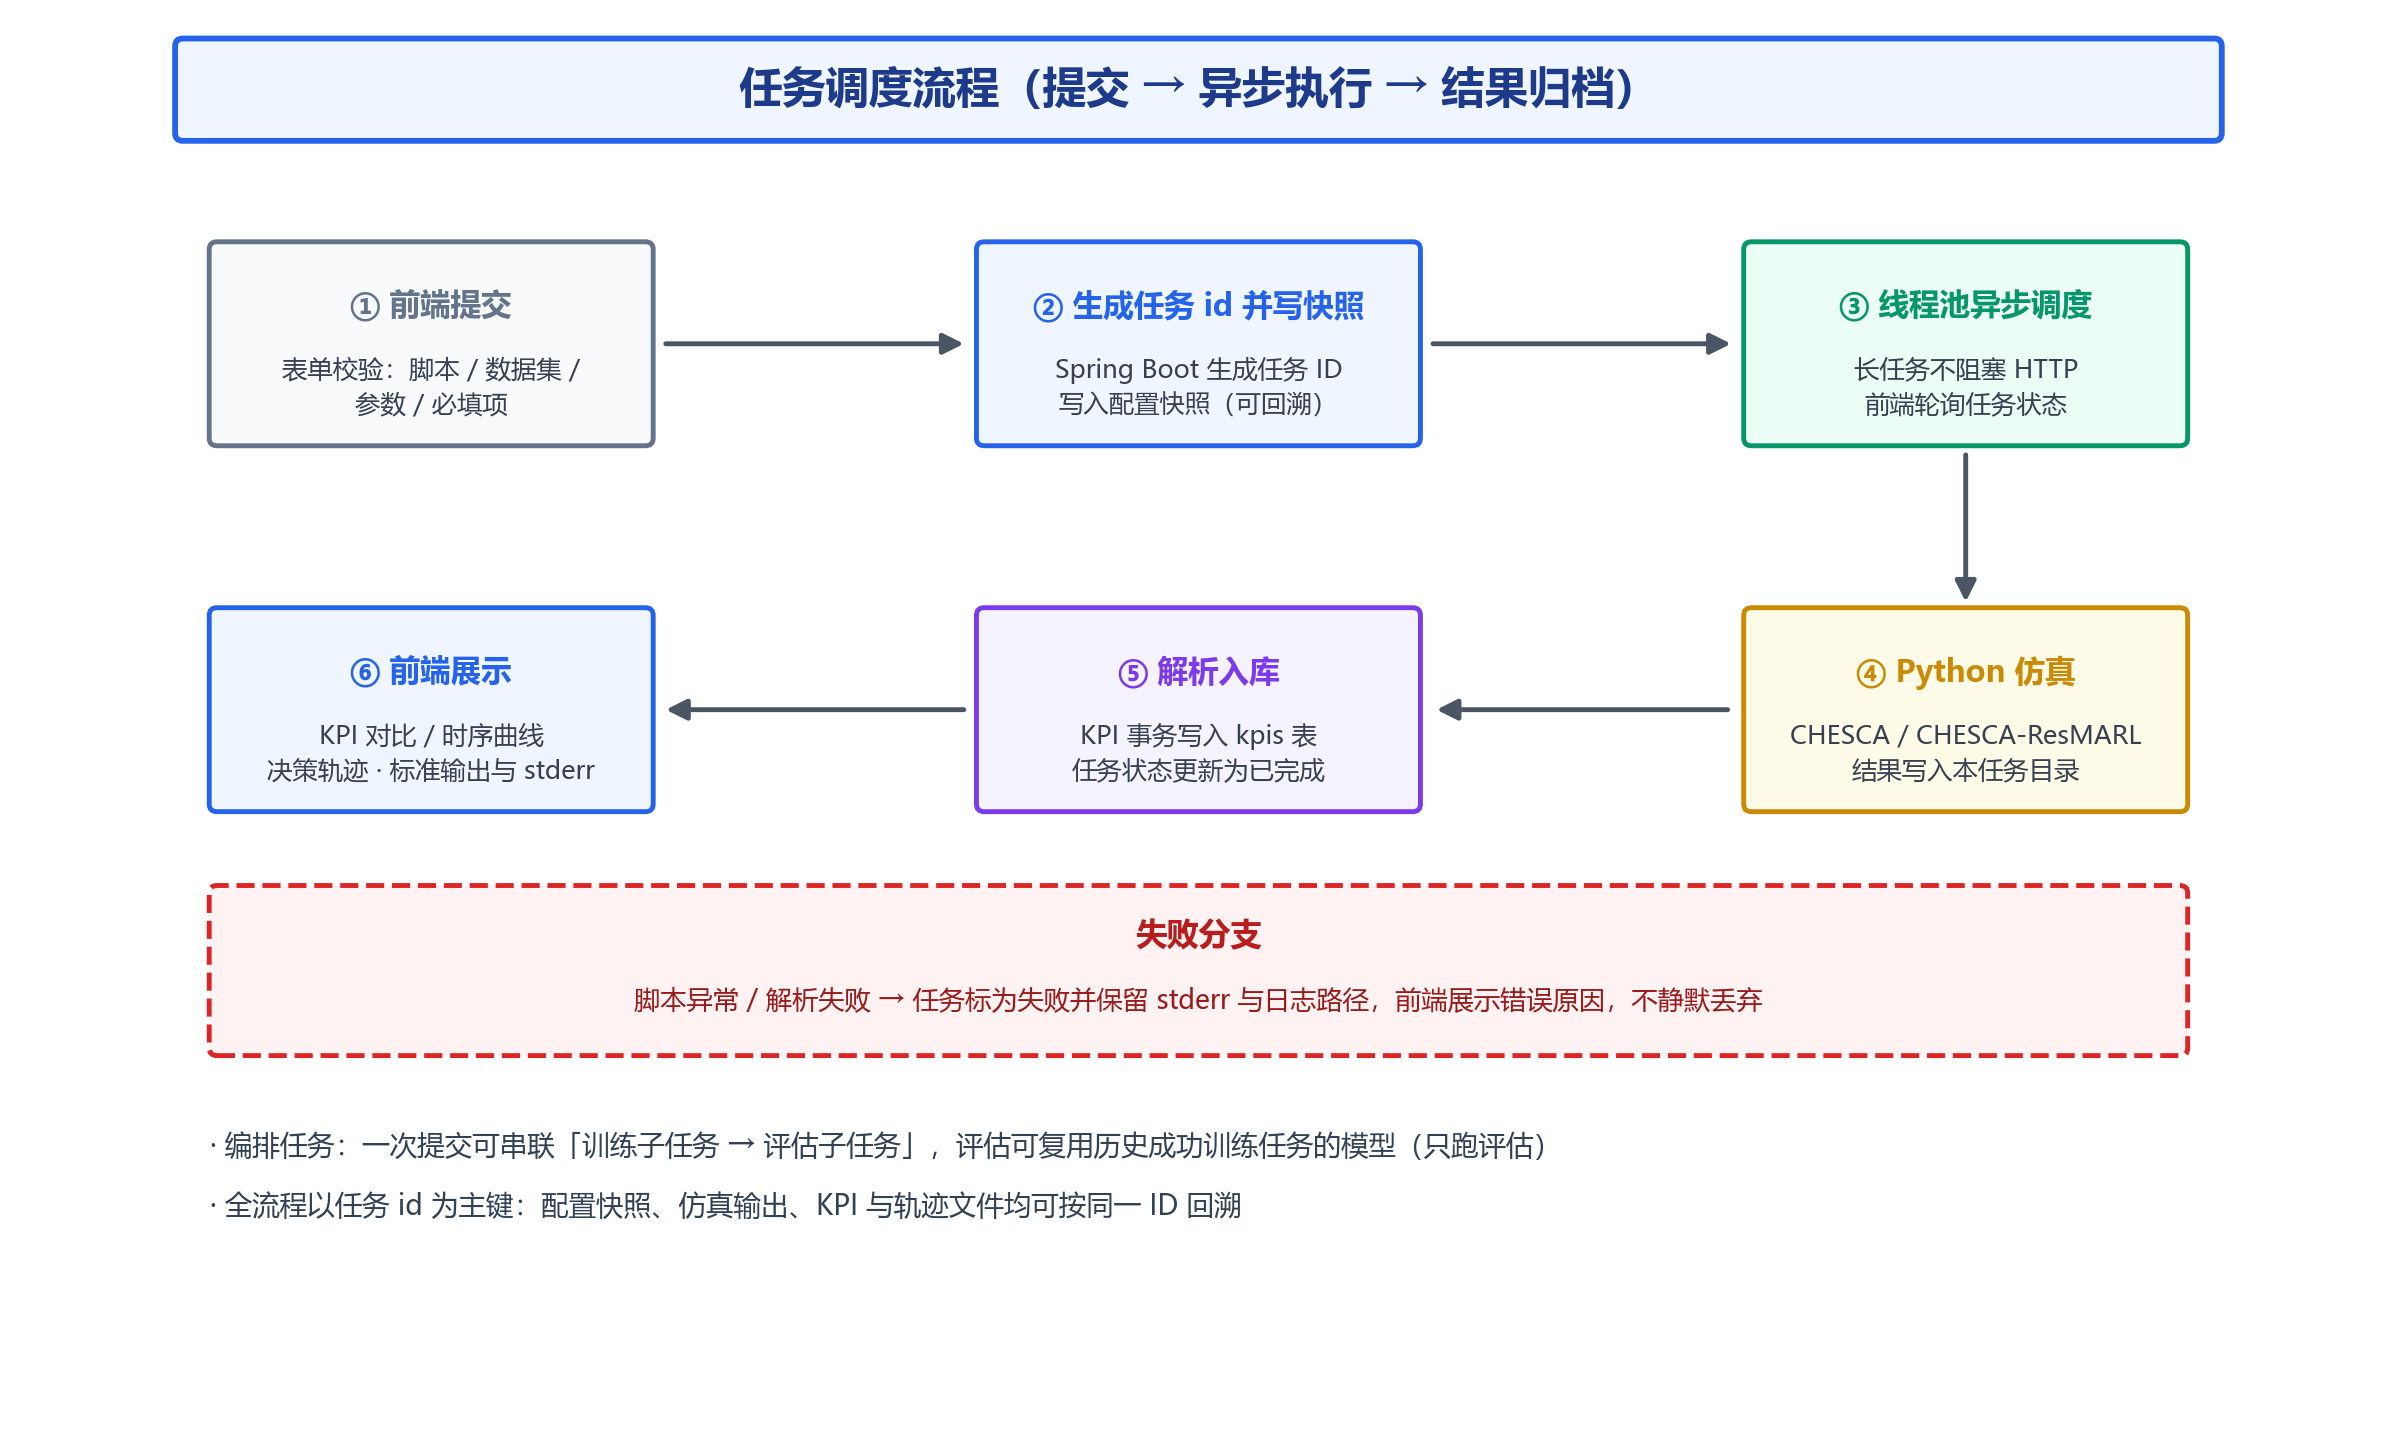
\includegraphics[width=0.90\textwidth]{./images/pictures/任务调度图.png}
    \centering\bicaption{任务调度图}{Task scheduling}
    \label{任务调度图}
\end{figure}

\begin{figure}[htb]
    \centering
    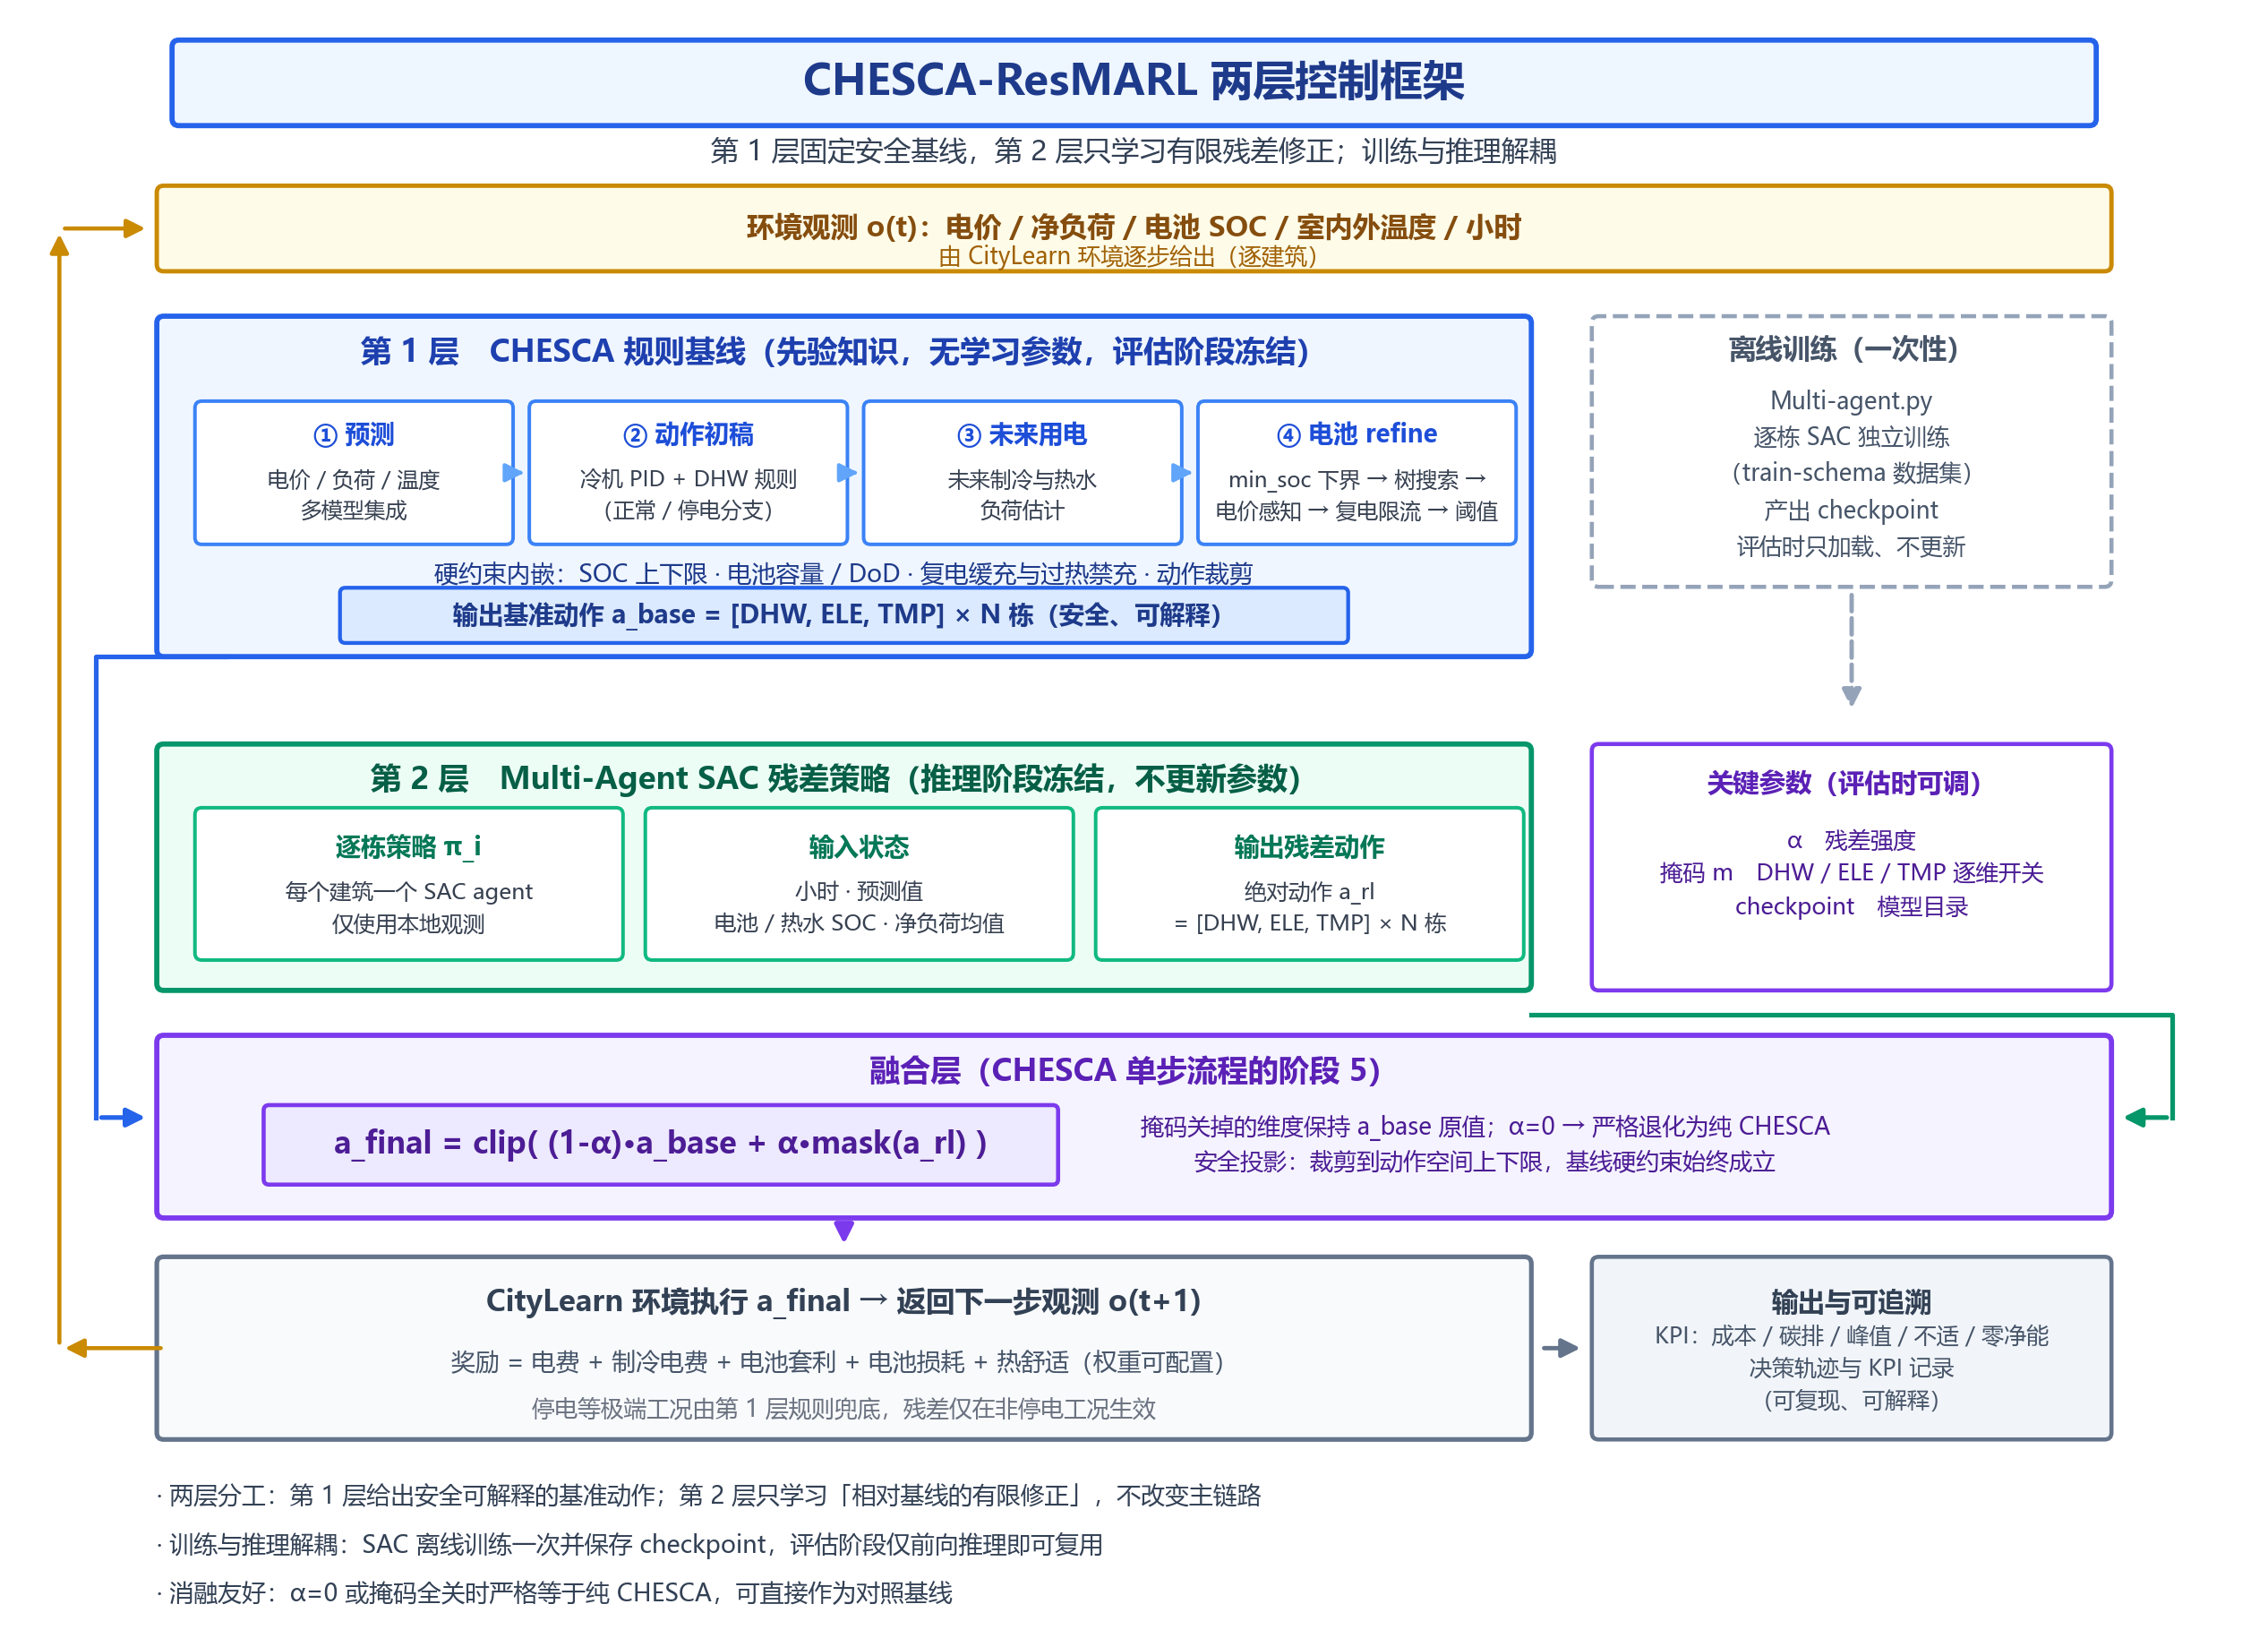
\includegraphics[width=0.85\textwidth]{./images/pictures/CHESCA-ResMARL框架.png}
    \centering\bicaption{CHESCA-ResMARL框架}{CHESCA-ResMARL framework}
    \label{CHESCA-ResMARL框架}
\end{figure}
残差合成过程如图\figref{残差合成图}所示。
\begin{figure}[htb]
    \centering
    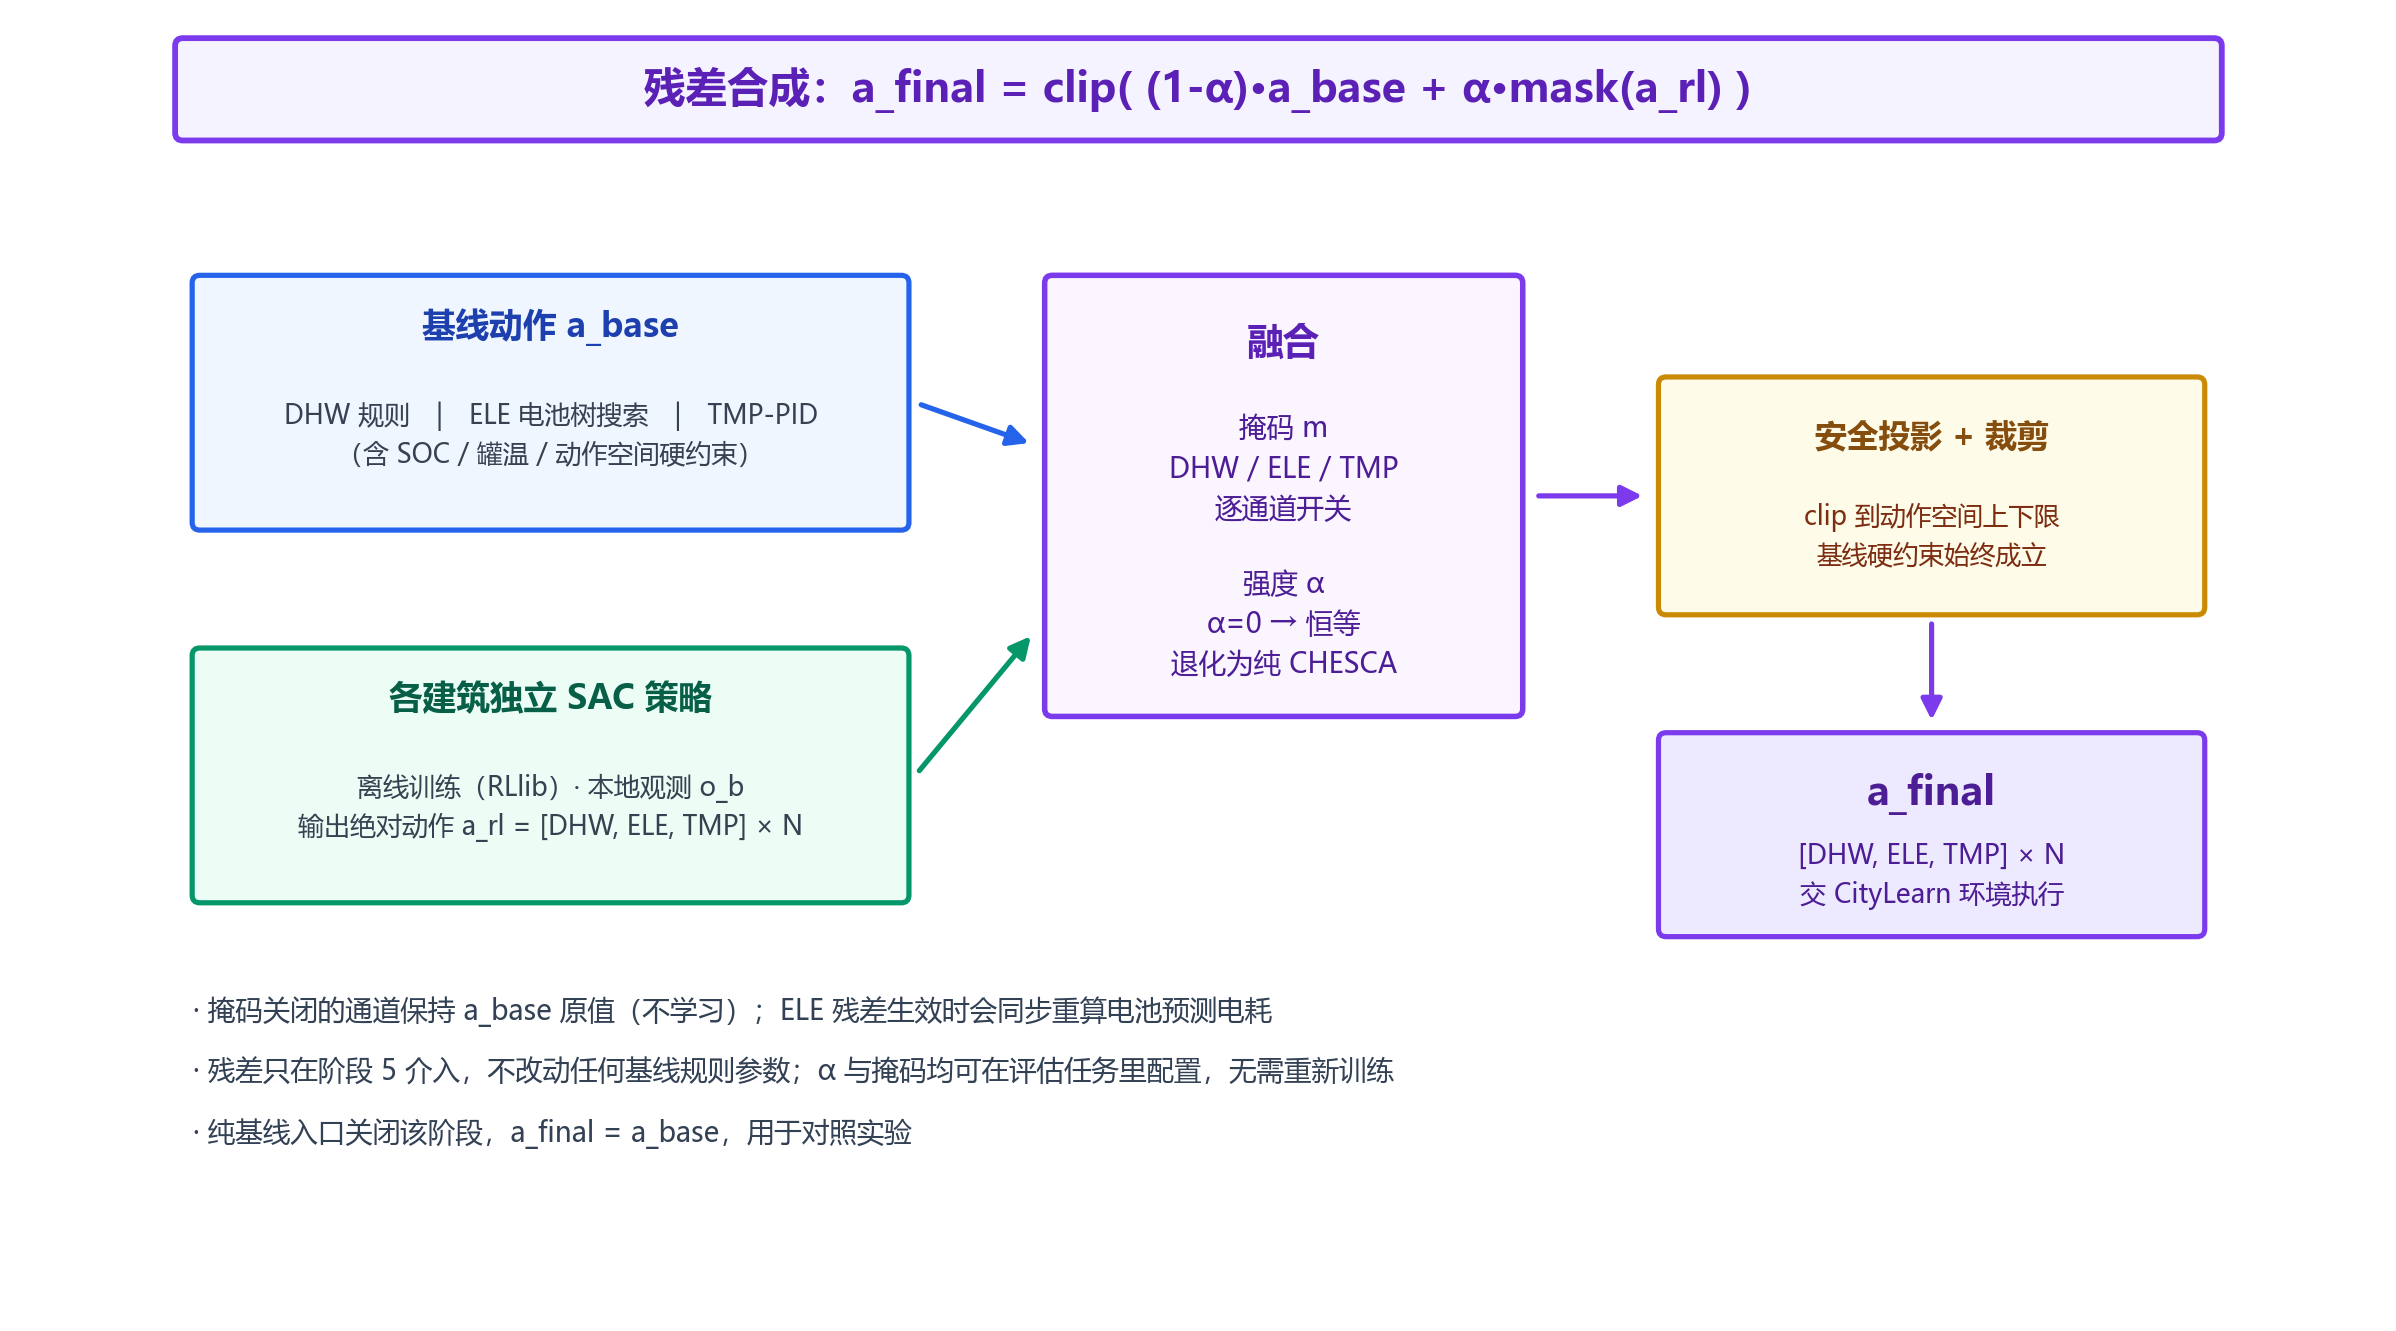
\includegraphics[width=0.92\textwidth]{./images/pictures/残差合成图.png}
    \centering\bicaption{残差合成图}{Residual fusion}
    \label{残差合成图}
\end{figure}

\section{前端系统功能介绍}
本节单独介绍前端系统功能，按``功能点+操作路径+界面截图''的方式组织，截图均取自平台实际运行界面。

\subsection{首页与导航}
功能：KPI卡片、新建任务快捷入口、通知入口。操作路径：登录进入首页，查看默认任务卡片，点击新建按钮跳转至配置页面。系统首页界面如图\ref{前端首页截图位}所示，包含导航栏、KPI卡片与新建任务快捷入口。
\begin{figure}[htb]
    \centering
    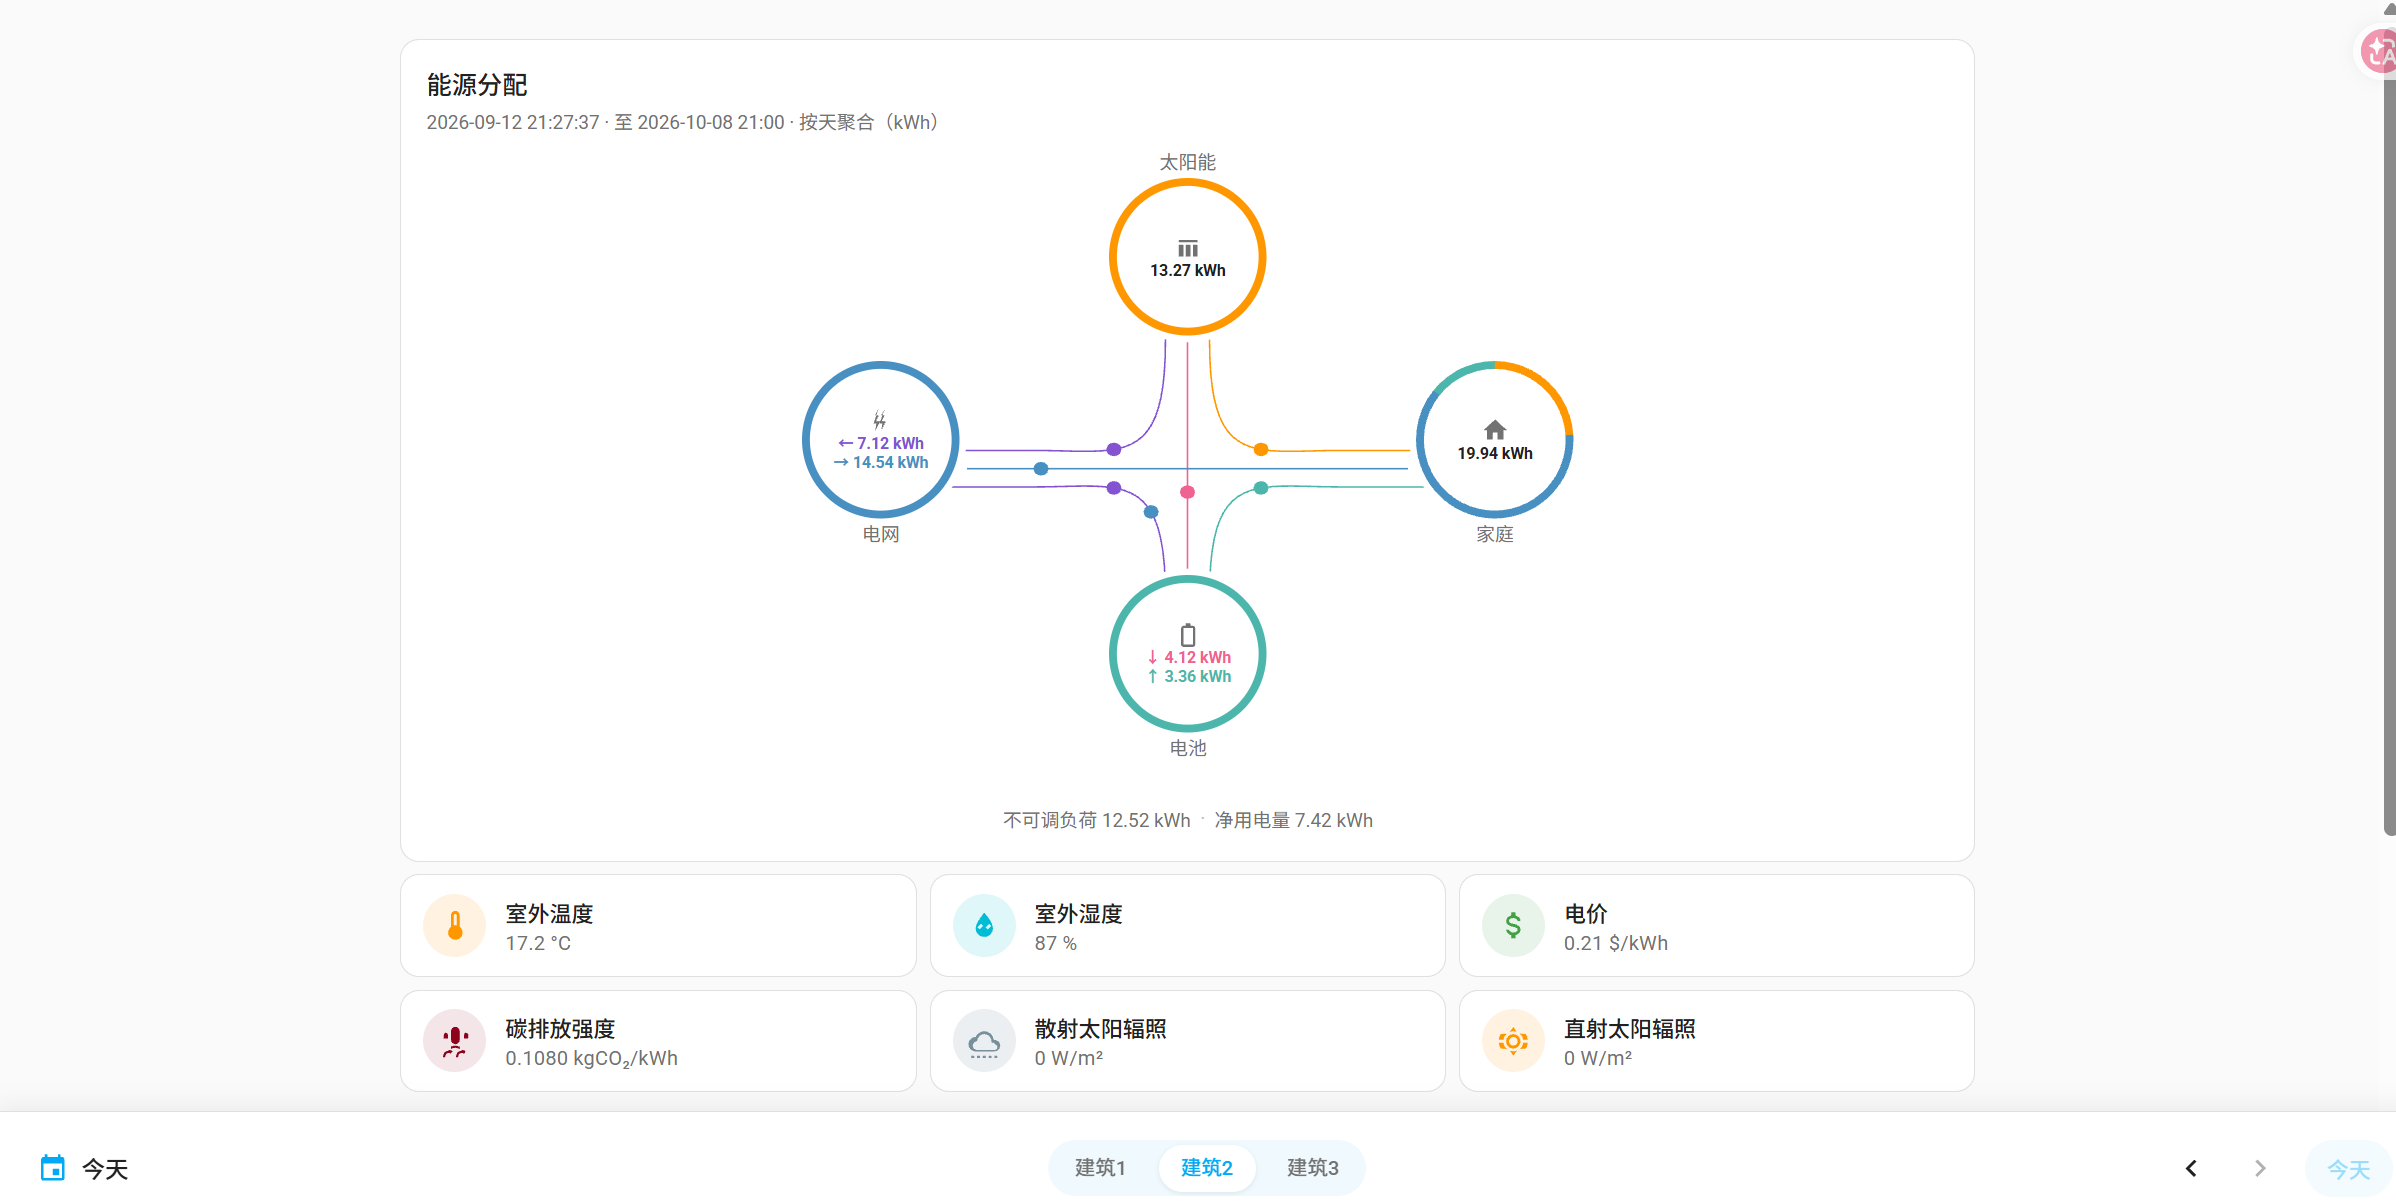
\includegraphics[width=0.85\textwidth]{./images/image/首页.jpg}
    \centering\bicaption{系统首页界面}{Frontend home}
    \label{前端首页截图位}
\end{figure}

\subsection{模型配置与任务提交}
功能：选择控制器、数据集、步数、残差系数、掩码、安全开关与模型文件，表单校验不通过时不发送请求。操作路径：在模型配置页填写参数并提交，在任务列表查看状态。算法配置界面如图\ref{前端配置截图位}所示，包含控制器、数据集、步数、残差系数、通道掩码、安全开关与模型文件等参数项，表单校验不通过时不发送请求。
\begin{figure}[htb]
    \centering
    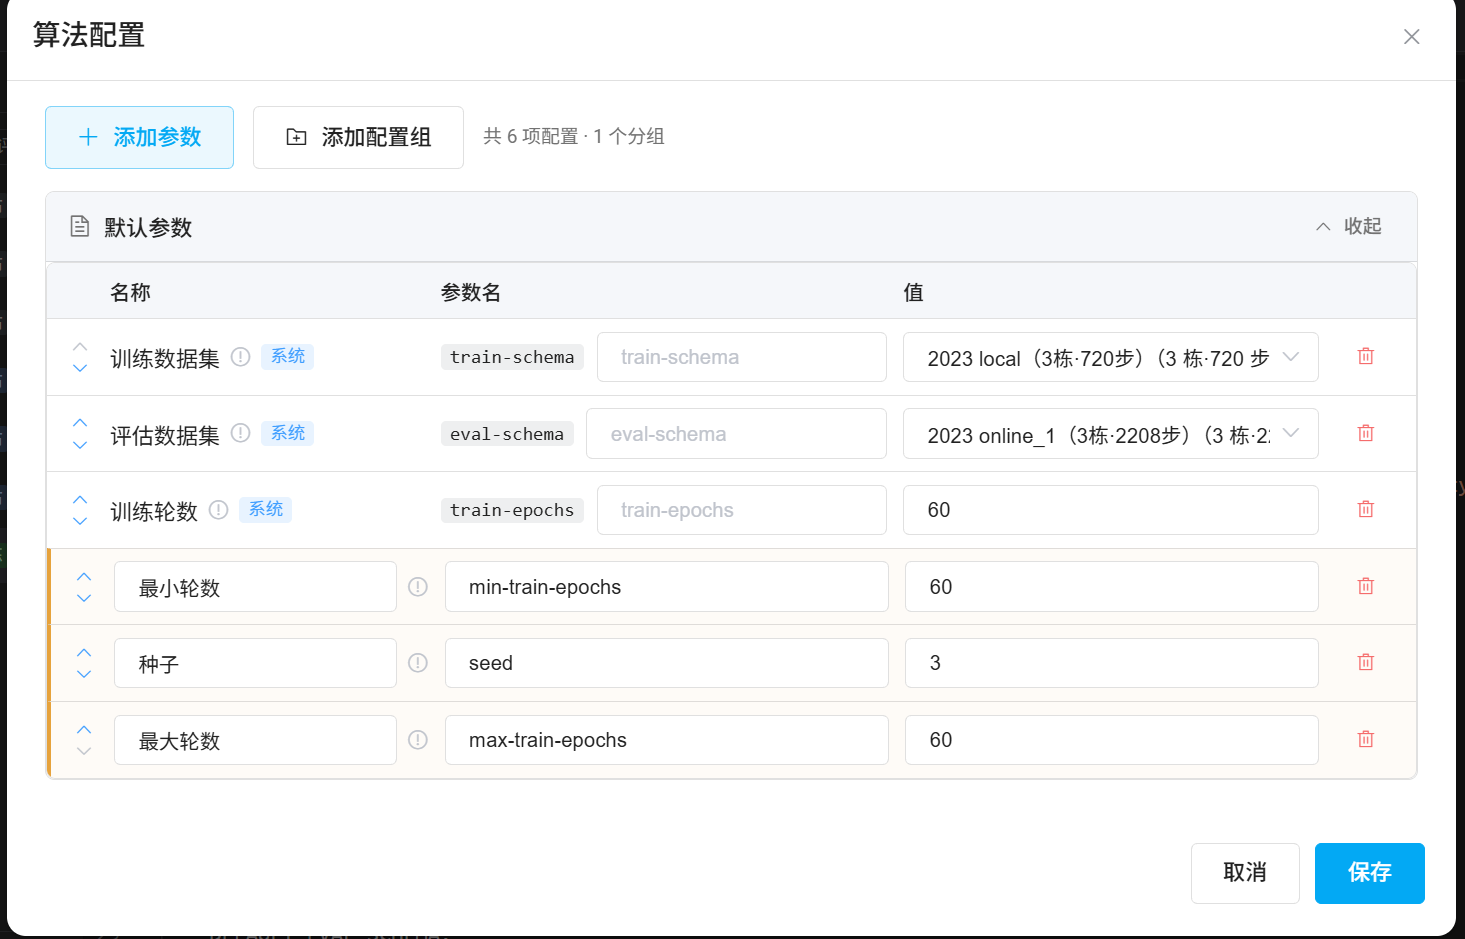
\includegraphics[width=0.85\textwidth]{./images/image/算法配置页.jpg}
    \centering\bicaption{算法配置页面}{Algorithm configuration page}
    \label{前端配置截图位}
\end{figure}

\subsection{能源分析与KPI对比}
功能：多任务KPI柱状图与雷达图、时序折线、任务检索。操作路径：在能源分析页输入任务标识，切换柱状/雷达/折线视图，对比无控制、CHESCA与残差策略。KPI指标对比界面如图\ref{前端KPI截图位}所示；原始数据查看页面支持按任务导出CSV时序数据，如图\ref{KPI对比图位}所示。
\begin{figure}[htb]
    \centering
    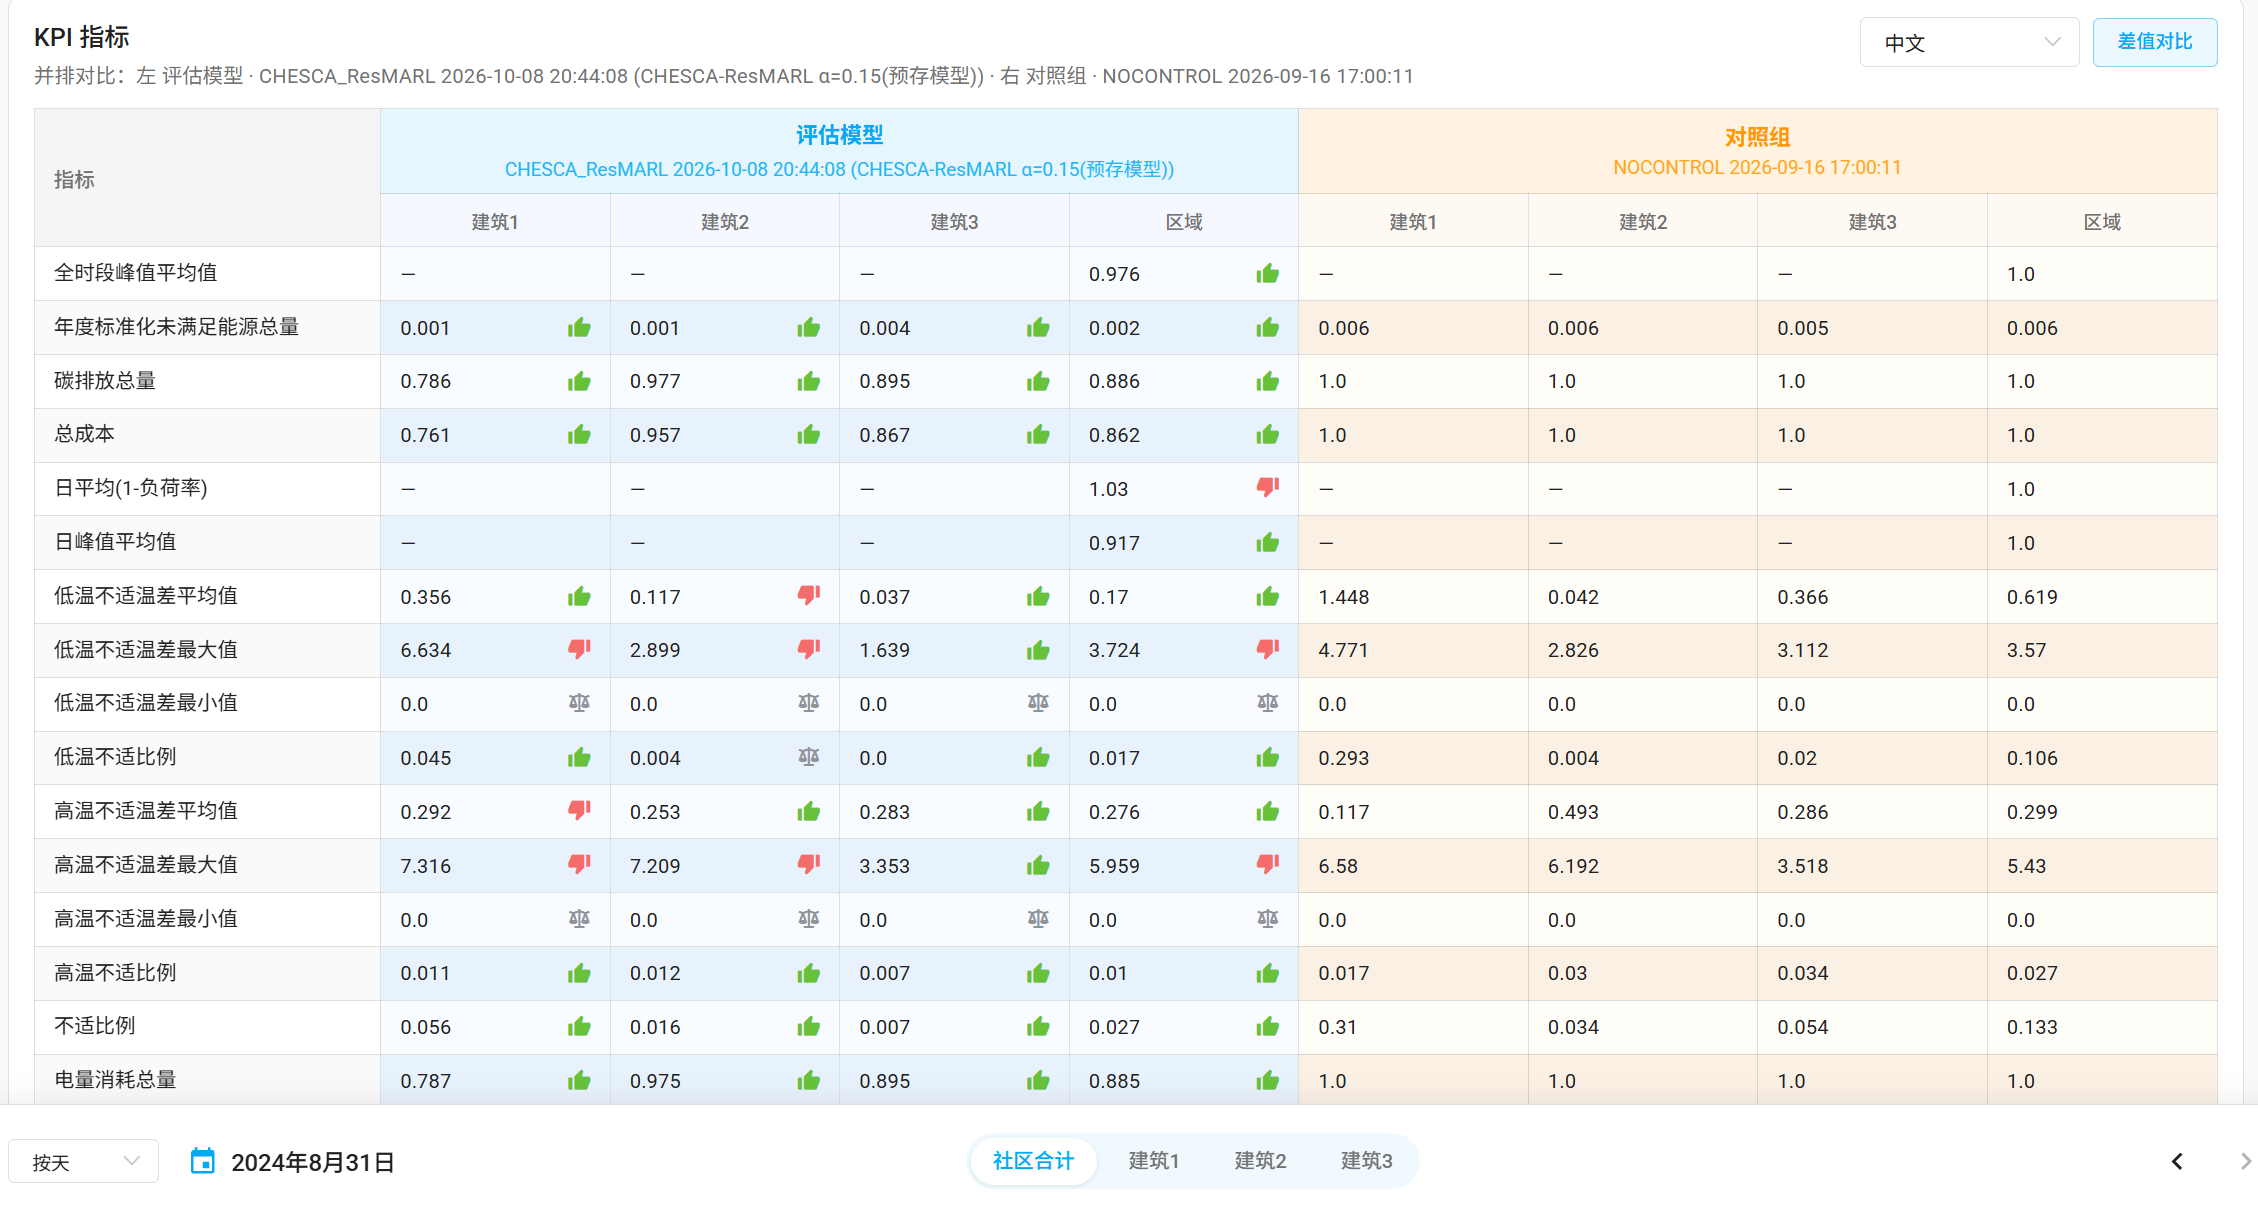
\includegraphics[width=0.85\textwidth]{./images/image/指标对比.jpg}
    \centering\bicaption{KPI指标对比页面}{KPI comparison}
    \label{前端KPI截图位}
\end{figure}
\begin{figure}[htb]
    \centering
    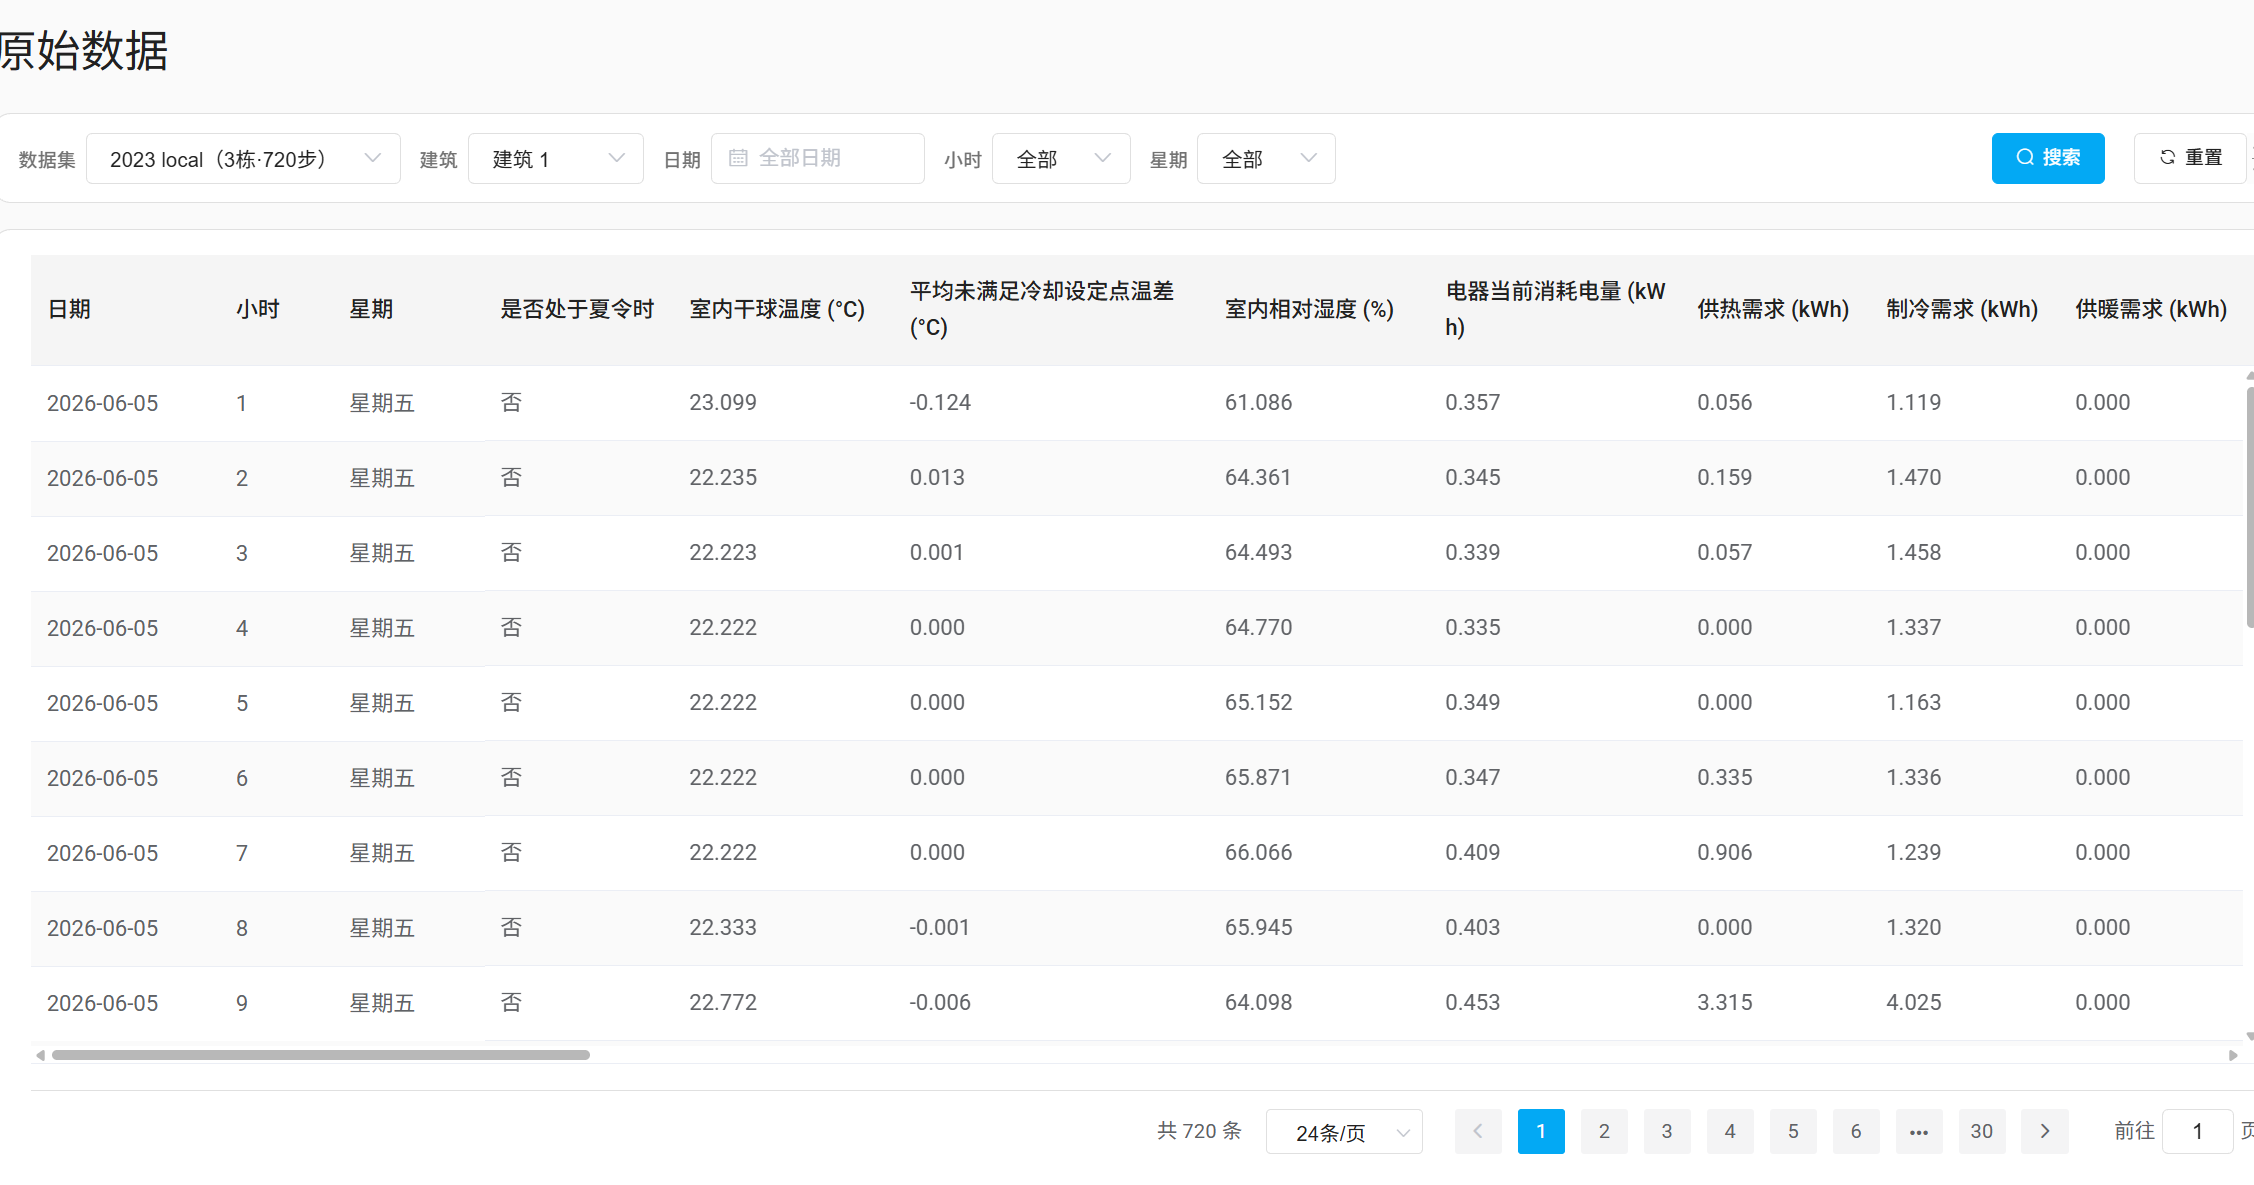
\includegraphics[width=0.85\textwidth]{./images/image/原始数据页.jpg}
    \centering\bicaption{原始数据查看页面}{Raw time-series data page}
    \label{KPI对比图位}
\end{figure}

\subsection{决策轨迹与残差查看}
功能：按时间步查看基线、残差、掩码、投影、SOC与舒适度状态，定位峰值时段。操作路径：在决策轨迹页输入任务标识与时间步，查看残差是否被安全层裁剪。决策轨迹页的环境状态面板如图\ref{前端轨迹截图位}与图\ref{环境状态动作截图位}所示，可查看室温、SOC与电价等状态量随时间步的变化。
\begin{figure}[htb]
    \centering
    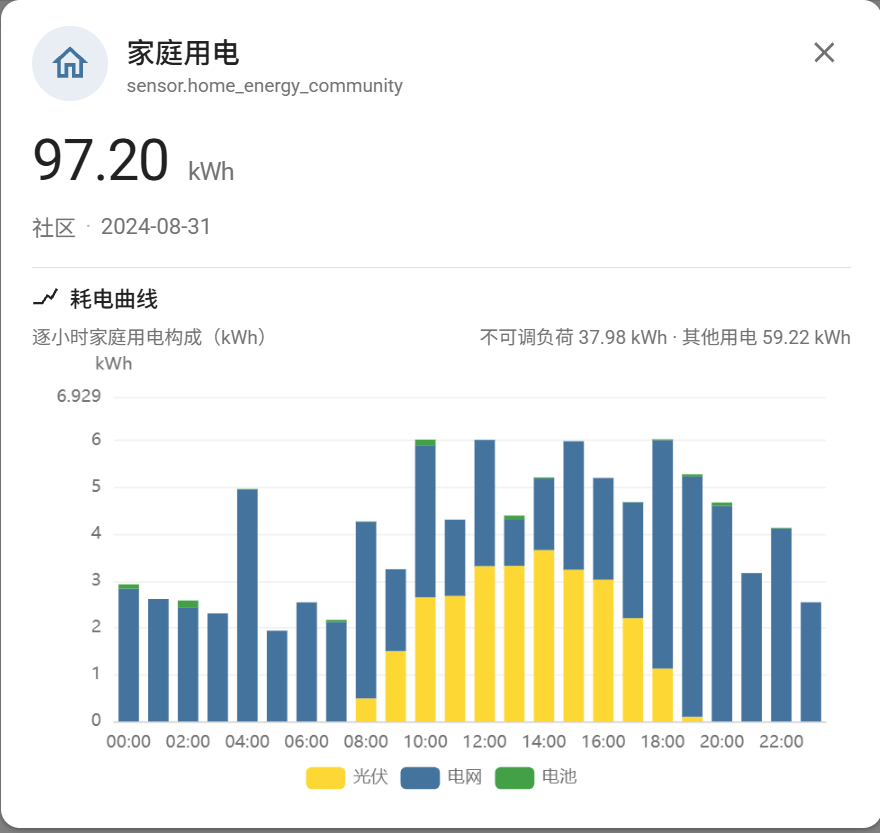
\includegraphics[width=0.85\textwidth]{./images/image/环境状态1.jpg}
    \centering\bicaption{决策轨迹环境状态（室温与SOC）}{Decision trace: temperature and SOC}
    \label{前端轨迹截图位}
\end{figure}
\begin{figure}[htb]
    \centering
    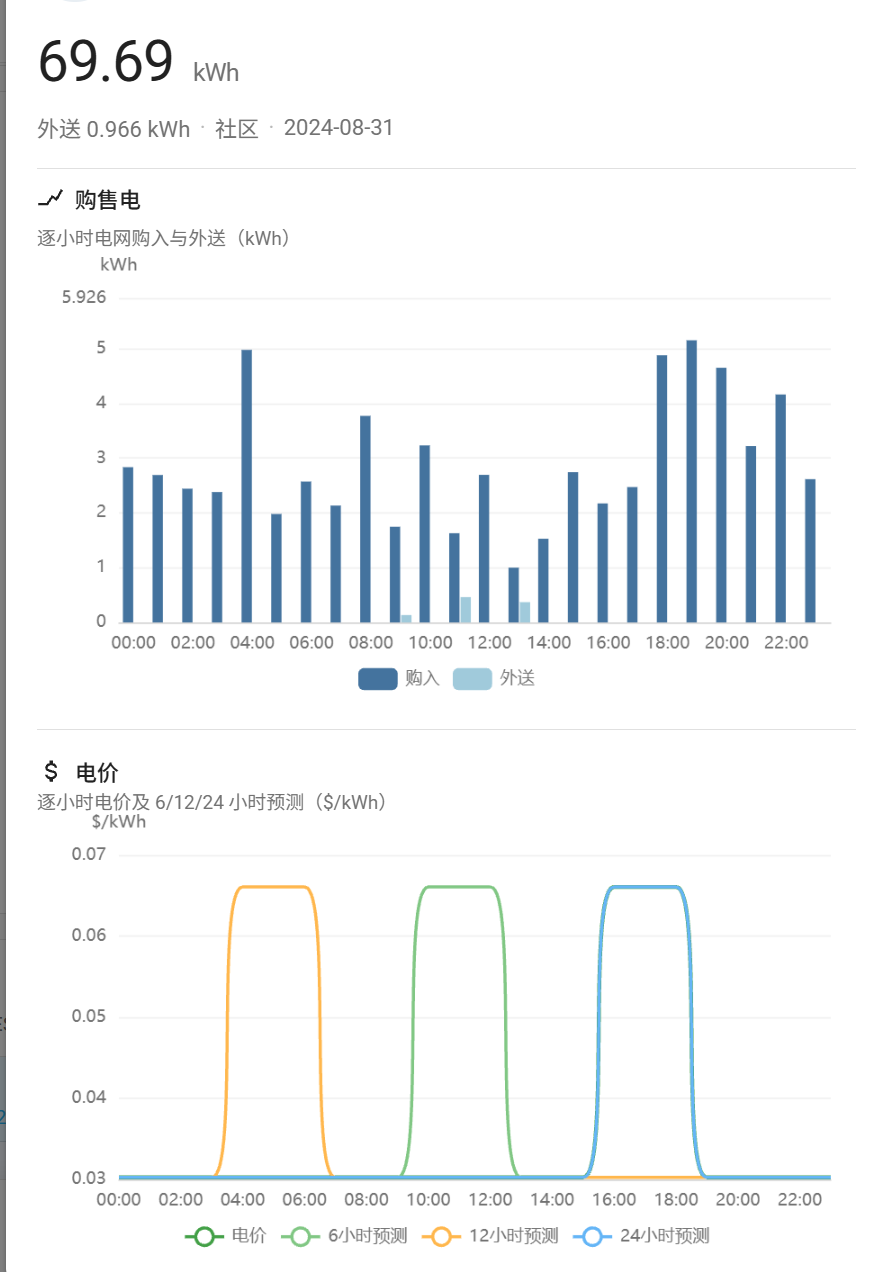
\includegraphics[width=0.85\textwidth]{./images/image/环境状态2-电价.jpg}
    \centering\bicaption{决策轨迹环境状态（电价）}{Decision trace: electricity price}
    \label{环境状态动作截图位}
\end{figure}

\subsection{其他页面与自动生成流程}
任务列表页面提供任务分页查询、进度跟踪与日志查看，菜单入口受权限控制；算法参数配置页面以分组表单维护各算法参数并内置在线代码编辑器，脚本编辑界面如图\ref{代码编辑器}所示；用户管理页面维护用户与角色；登录页面完成身份认证与跳转。此外，系统还提供了残差系数敏感性分析、预测误差展示与各通道残差分布展示等辅助视图。任务管理自动化流程如图\ref{自动可视化流程占位}所示，覆盖从数据集准备、训练、评估到指标入库的完整链路；残差调优流程以示意图形式给出。
\begin{figure}[htb]
    \centering
    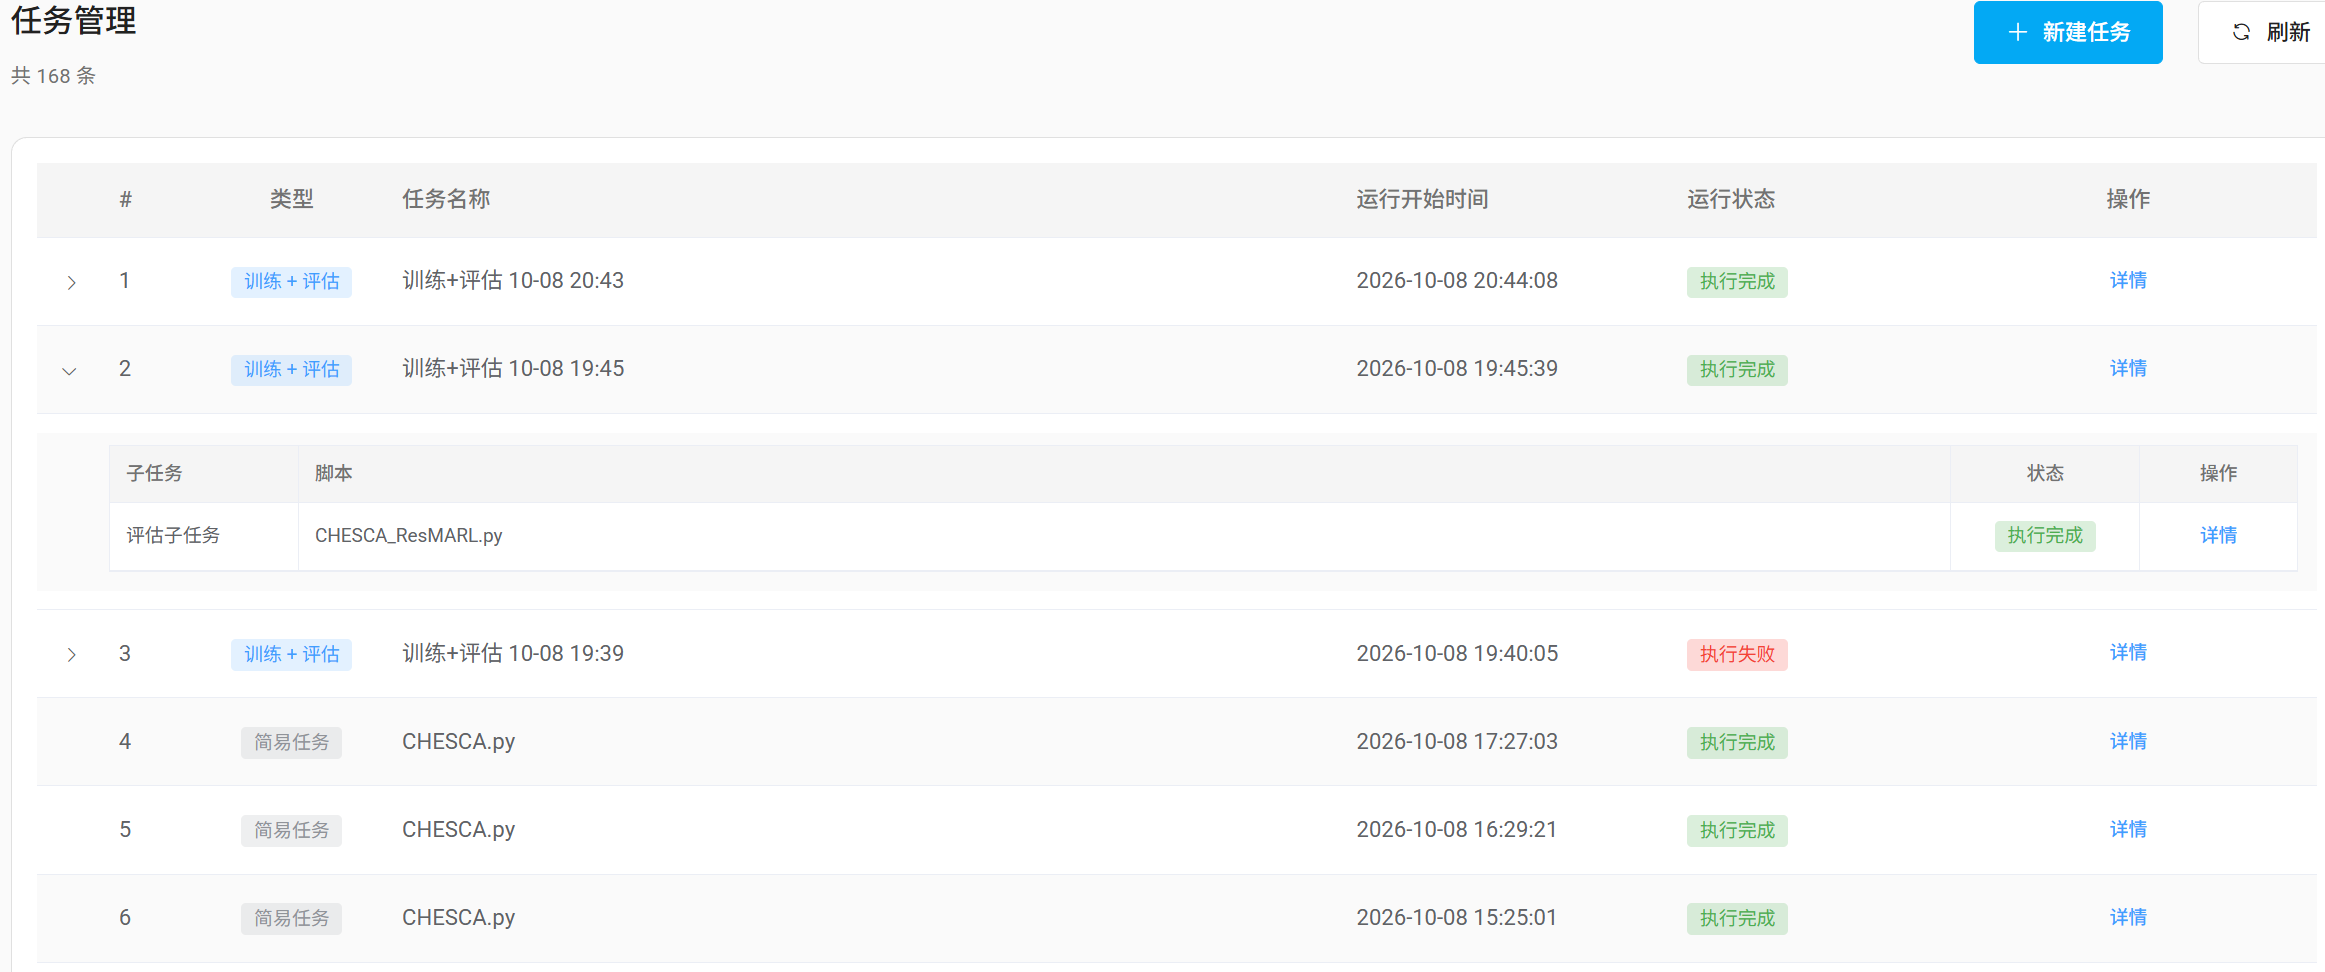
\includegraphics[width=0.8\textwidth]{./images/image/任务管理自动化流程.jpg}
    \centering\bicaption{任务管理自动化流程}{Task management automation pipeline}
    \label{自动可视化流程占位}
\end{figure}
\begin{figure}[htb]
    \centering
    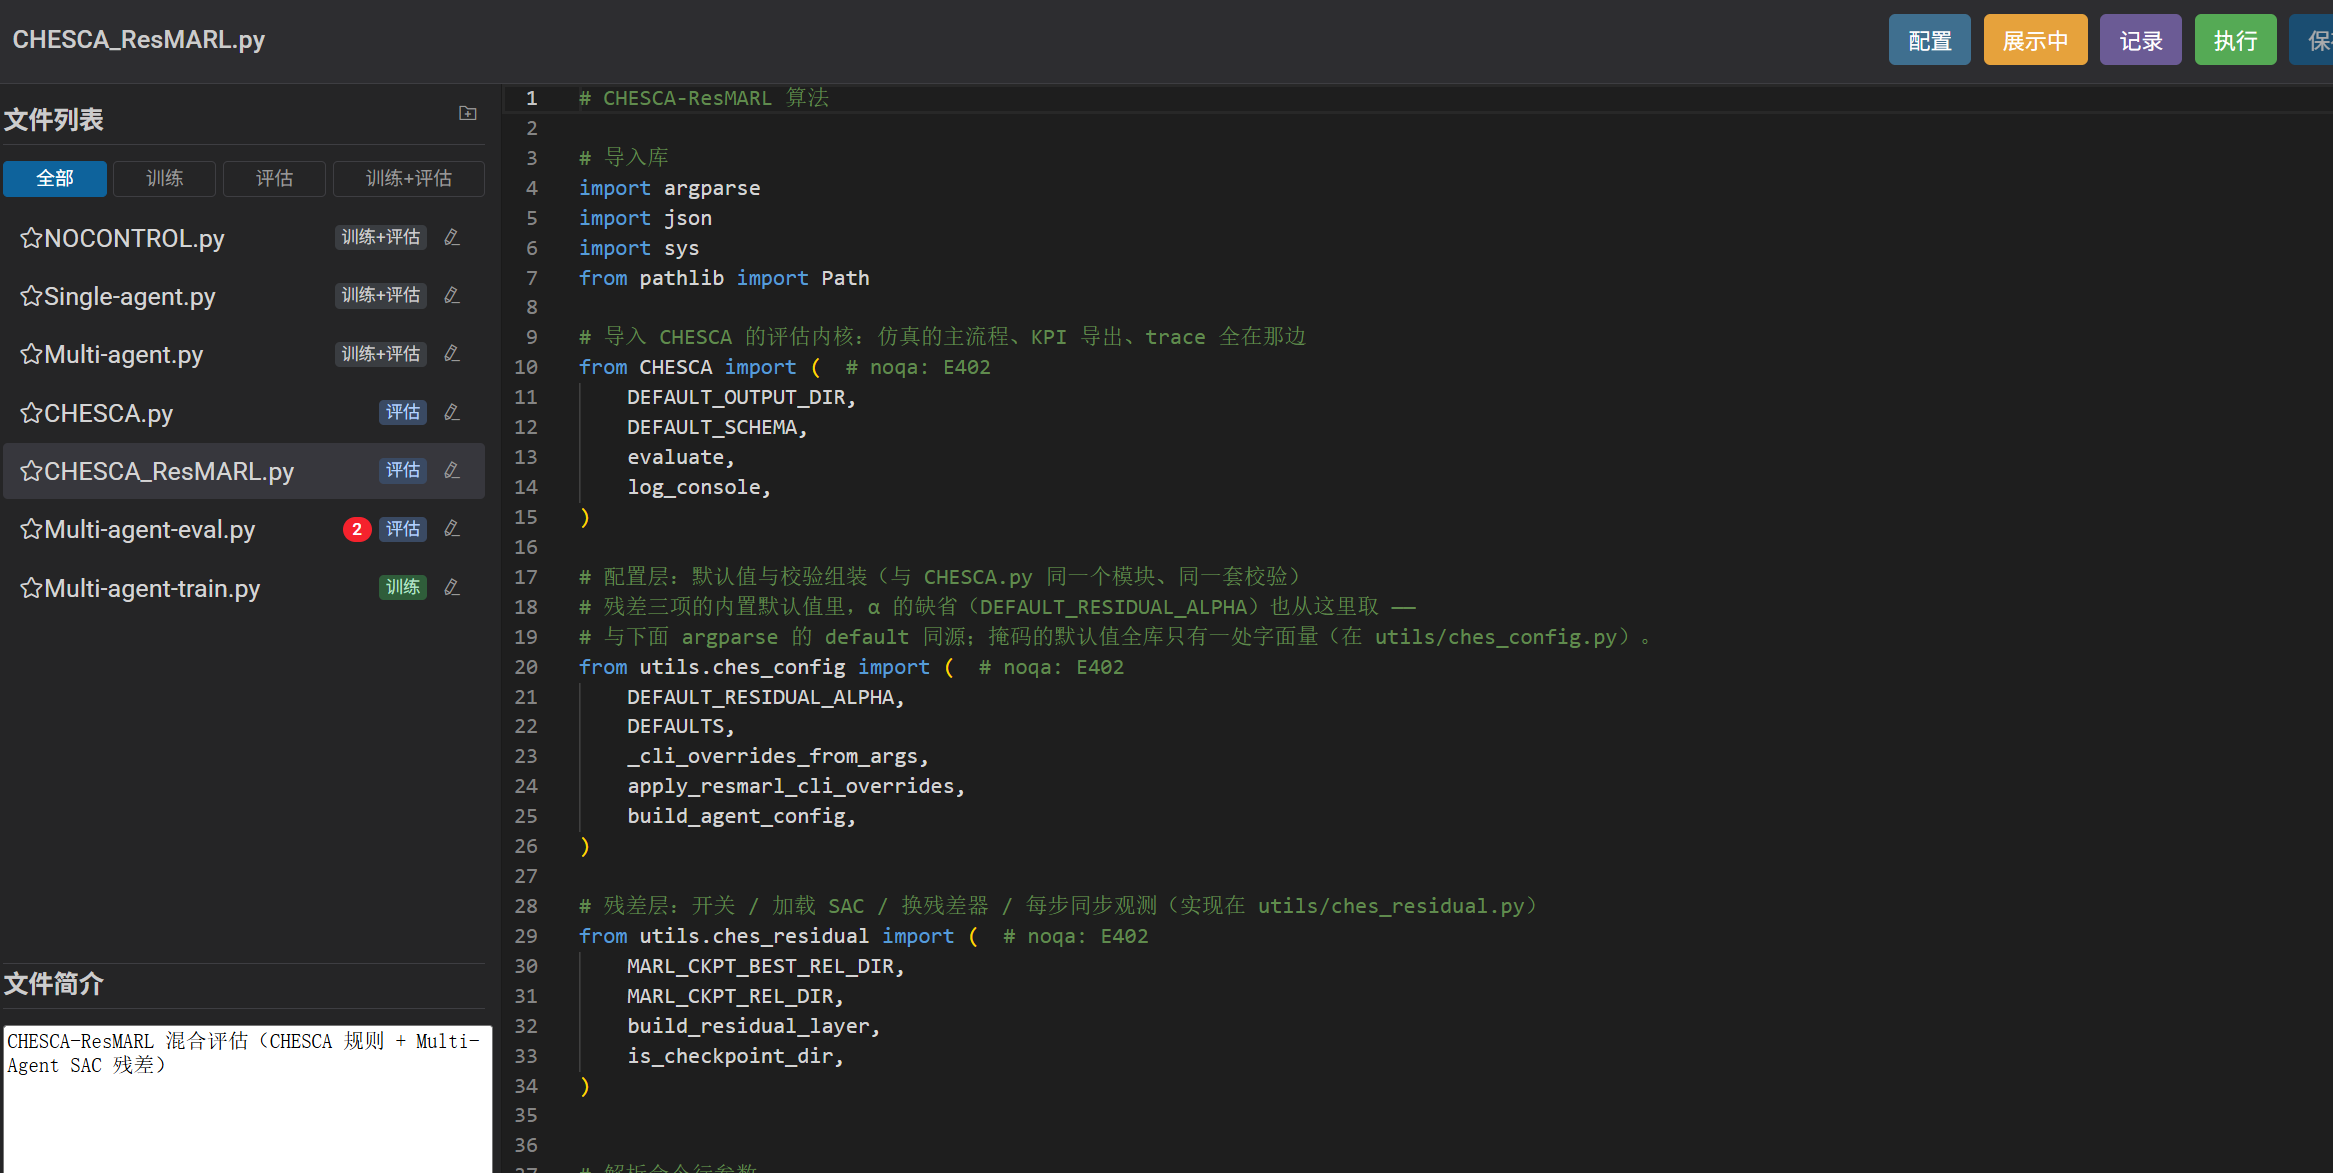
\includegraphics[width=0.85\textwidth]{./images/image/代码编辑器.jpg}
    \centering\bicaption{算法参数配置与脚本编辑界面}{Algorithm parameter configuration and script editing}
    \label{代码编辑器}
\end{figure}
\begin{figure}[htb]
    \centering
    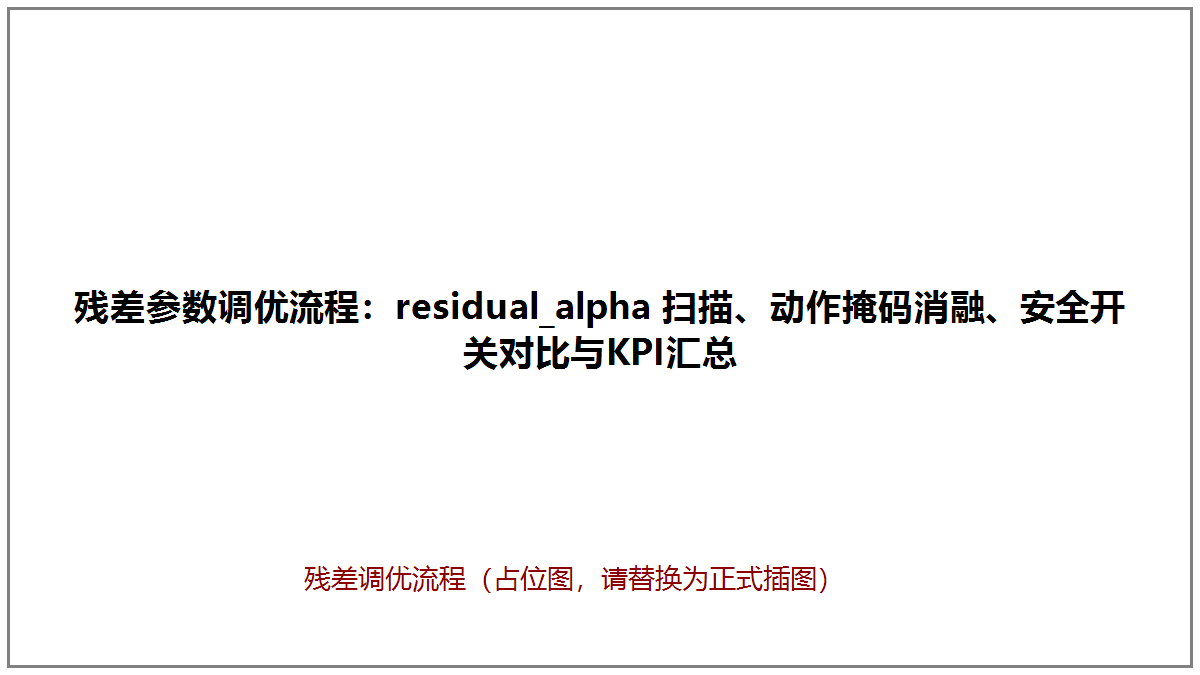
\includegraphics[width=0.8\textwidth]{./images/pictures/残差调优流程.png}
    \centering\bicaption{残差调优流程}{Residual tuning workflow}
    \label{残差调优流程占位}
\end{figure}

\section{本章小结}
本章将系统设计落地为具体实现：页面部分阐述布局与校验逻辑，日志部分说明当前组合方案与ELK备选，存储部分介绍五组数据表与索引设计，调度部分说明任务标识贯通全链路的机制，前端部分单列章节介绍界面功能。下一章将通过Postman契约测试、功能用例与CityLearn消融实验对上述内容进行验证。
